\documentclass[11pt]{report}
\usepackage[german, english]{babel}
\usepackage{geometry}                % See geometry.pdf to learn the layout options. There are lots.
\geometry{a4paper}                   % ... or a4paper or a5paper or ... 
%\usepackage[parfill]{parskip}    % Activate to begin paragraphs with an empty line rather than an indent
\usepackage{xifthen}
\usepackage{xstring}			% to check content of strings in xifthen
\usepackage{graphicx}
\usepackage[usenames,dvipsnames,table]{xcolor}
\usepackage{amssymb}
\usepackage{epstopdf}
\usepackage[utf8]{inputenc}
\usepackage{hyperref}
\usepackage{fancyhdr}
\setcounter{tocdepth}{4}
\setcounter{secnumdepth}{4}

\IfStrEq*{\languagename}{english}
	{
		\newcommand{\dalabel}{Diploma Thesis}
		\newcommand{\submittedlabel}{Submitted by}
		\newcommand{\datelabel}{Date}
		\newcommand{\supervisorlabel}{Supervisor}
		\newcommand{\projectpartnerlabel}{Project Partner}
	}
	{
		\newcommand{\dalabel}{Diplomarbeit}
		\newcommand{\submittedlabel}{Eingereicht von}
		\newcommand{\datelabel}{Datum}
		\newcommand{\supervisorlabel}{Betreuer}
		\newcommand{\projectpartnerlabel}{Projektpartner}
	}
 % This file should not really be touched
\newcommand{\titleofthesis}{Writing the \LaTeX{} Way under consideration of long titles which must not spoil the title page}
\newcommand{\department}{Medientechnik} % Replace by your department

\newcommand{\firstauthor}{Peter Bauer}
\newcommand{\firstauthorclass}{5AHIF}
\newcommand{\secondauthor}{Richard Kainerstorfer}
\newcommand{\secondauthorclass}{5BHIF}
\newcommand{\thirdauthor}{Alfred Wiedermann}
\newcommand{\thirdauthorclass}{5AHBG}
\newcommand{\fourthauthor}{Wolfgang Holzer}
\newcommand{\fourthauthorclass}{5AHEL}

\newcommand{\duedateen}{April 4, 2018} % due date in english format
\newcommand{\duedatede}{4. April 2018} % due date in german format
\newcommand{\supervisor}{Peter Bauer}
\newcommand{\projectpartner}{MathConsult}
 % Set basic data (author, title, etc.) of your thesis
\begin{document}
\rhead{
\includegraphics[scale=.9]{images/Logo.png}}
\cfoot{}
\begin{titlepage}
\thispagestyle{fancy}

\begin{center}

\vspace*{8em}

{\LARGE \dalabel}

\vspace{2em}

{\large Höhere Technische Bundeslehranstalt Leonding \\[.5em]
Abteilung für \department}

%\vspace{8em}
\vspace*{\fill}

{\Huge \titleofthesis}
\end{center}

%\vspace{8em}
\vspace*{\fill}

\begin{tabular}{ll}
\ifthenelse{\isundefined{\firstauthor}}{}{\submittedlabel: & {\bf \firstauthor, \firstauthorclass}}
\ifthenelse{\isundefined{\secondauthor}}{}{ \\[.5em] & {\bf \secondauthor, \secondauthorclass}}
\ifthenelse{\isundefined{\thirdauthor}}{}{ \\[.5em] & {\bf \thirdauthor, \thirdauthorclass}}
\ifthenelse{\isundefined{\fourthauthor}}{}{ \\[.5em] & {\bf \fourthauthor, \fourthauthorclass}}
 \\[.5em]
\datelabel: & {\bf \duedateen} \\[.5em]

\supervisorlabel: & {\bf \supervisor} \\[.5em]

\ifthenelse{\isundefined{\projectpartner}}{}{\projectpartnerlabel: & {\bf \projectpartner}}
\end{tabular}
\end{titlepage}
 % Should not be necessary to touch this file
\section*{Declaration of Academic Honesty}
Hereby, I declare that I have composed the presented paper independently on my own and without any other resources than the ones indicated. All thoughts taken directly or indirectly from external sources are properly denoted as such.

This paper has neither been previously submitted to another authority nor has it been published yet. \\[1em]
Leonding, \duedateen \\[5em]
\ifthenelse{\isundefined{\firstauthor}}{}{\firstauthor}
\ifthenelse{\isundefined{\secondauthor}}{}{\kern-1ex, \secondauthor}
\ifthenelse{\isundefined{\thirdauthor}}{}{\kern-1ex, \thirdauthor}
\ifthenelse{\isundefined{\fourthauthor}}{}{\kern-1ex, \fourthauthor} \\[5em]

\begin{otherlanguage}{german}
\section*{Eidesstattliche Erklärung}
Hiermit erkläre ich an Eides statt, dass ich die vorgelegte Diplomarbeit selbstständig und ohne Benutzung anderer als der angegebenen Hilfsmittel angefertigt habe. Gedanken, die aus fremden Quellen direkt oder indirekt übernommen wurden, sind als solche gekennzeichnet.

Die Arbeit wurde bisher in gleicher oder ähnlicher Weise keiner anderen Prüfungsbehörde vorgelegt und auch noch nicht veröffentlicht. \\[1em]
Leonding, am \duedatede \\[5em]
\ifthenelse{\isundefined{\firstauthor}}{}{\firstauthor}
\ifthenelse{\isundefined{\secondauthor}}{}{\kern-1ex, \secondauthor}
\ifthenelse{\isundefined{\thirdauthor}}{}{\kern-1ex, \thirdauthor}
\ifthenelse{\isundefined{\fourthauthor}}{}{\kern-1ex, \fourthauthor} \\[5em]
\end{otherlanguage}

\begin{abstract}
Here it is described what the thesis is all about. The abstract shall be brief and concise and its size  shall not go beyond one page. Furthermore it has no chapters, sections etc. Paragraphs can be used to structure the abstract. If necessary one can also use bullet point lists but care must be taken that also in this part of the text full sentences and a clearly readable structure are required.

Concerning the content the following points shall be covered. 

\begin{enumerate}
	\item {\em Definition of the project:} What do we currently know about the topic or on which results can the work be based? What is the goal of the project? Who can use the results of the project?
	
	\item {\em Implementation:} What are the tools and methods used to implement the project?
	
	\item {\em Results:} What is the final result of the project?
\end{enumerate}
This list does not mean that the abstract must strictly follow this structure. Rather it should be understood in that way that these points shall be described such that the reader is animated  to dig further into the thesis.

Finally it is required to add a representative image which describes your project best. The image here shows Leslie Lamport the inventor of \LaTeX.

\begin{flushright}
	\includegraphics[scale=.25]{images/leslie_lamport.jpg}
\end{flushright}

\end{abstract}

\begin{otherlanguage}{german}
\begin{abstract}
An dieser Stelle wird beschrieben, worum es in der Diplomarbeit geht. Die Zusammenfassung soll kurz und prägnant sein und den Umfang einer Seite nicht übersteigen. Weiters ist zu beachten, dass hier keine Kapitel oder Abschnitte zur Strukturierung verwendet werden. Die Verwendung von Absätzen ist zulässig. Wenn notwendig, können auch Aufzählungslisten verwendet werden. Dabei ist aber zu beachten, dass auch in der Zusammenfassung vollständige Sätze gefordert sind.

Bezüglich des Inhalts sollen folgende Punkte in der Zusammenfassung vorkommen: 

\begin{itemize}
	\item {\em Aufgabenstellung:} Von welchem Wissenstand kann man im Umfeld der Aufgabenstellung ausgehen? Was ist das Ziel des Projekts? Wer kann die Ergebnisse der Arbeit benutzen?
	
	\item {\em Umsetzung:} Welche fachtheoretischen oder -praktischen Methoden wurden bei der Umsetzung verwendet?
	
	\item {\em Ergebnisse:} Was ist das endgültige Ergebnis der Arbeit?
\end{itemize}
Diese Liste soll als Sammlung von inhaltlichen Punkten für die Zusammenfassung verstanden werden. Die konkrete Gliederung und Reihung der Punkte ist den Autoren überlassen. Zu beachten ist, dass der/die LeserIn beim Lesen dieses Teils Lust bekommt, diese Arbeit weiter zu lesen.

Abschließend soll die Zusammenfassung noch ein Foto zeigen, das das beschriebene Projekt am besten repräsentiert. Das folgende Bild zeigt Leslie Lamport, den Erfinder von \LaTeX.

\begin{flushright}
	\includegraphics[scale=.25]{images/leslie_lamport.jpg}
\end{flushright}

\end{abstract}
\end{otherlanguage}

\section*{Acknowledgments}
If you feel like saying thanks to your grandma and/or other relatives.
 % Declaration of Academic Honesty, Abstracts, Acknowledgments, 
\begin{otherlanguage}{german}
    

\tableofcontents


\chapter{Introduction}
\section{Initial Situation}
Klassische Brettspiele benötigen viel Platz zum Verstauen. Platz welche eine Familie eventuell nicht mal daheim hat, aber schon gar nicht wenn sie in die Ferien fahren. Brettspiele benötigen viel zu viel Platz im Koffer und man muss sich, wenn man schon welche mitnimmt, für ein paar wenige entscheiden. Und wenn dem Kind dann zufällig die Spiele gerade nicht passen hat man ein Problem. Bei Ludimus hat man die komplette Spielesammlung in der Cloud und kann sie immer und überall mitnehmen ohne viel Platz zu brauchen.
\newline 
Auch werden Kinder immer abgeneigter gegenüber klassischen Brettspielen und wollen lieber was am Handy spielen. Mithilfe von Ludimus können Eltern das Spielen mit ihren Kindern mit dem,  lieber am Handy spielen ihrer Kinder verbinden, da die Plattform komplett über das Smartphone gesteuert wird.

\section{Goals}
The general goals and objectives of the project are described here. Care must be taken that the goals documented here are purely project goals and have nothing to do with individual goals of the team members. If individual goals should be part of the thesis they are listed in appendix~\ref{cha:individual-goals}.

\section{Overview}
Details of the diploma thesis have to be aligned between student and supervisor. This should be a basic structure to facilitate the first steps when students start to write their theses.

Never forget to add some illustrative images. Images must not be messed up with your normal text. They are encapsulated in floating bodies and referenced in your text. An example can be seen in figure~\ref{fig:sample}. As you can see, figures are placed by default on top of the page nearby the place where they are referenced the first time. Furthermore you can see that a list of figures is maintained automatically which can be included easily by typing the command \verb1\listoffigures1 into your document.

\begin{figure}
\begin{center}
	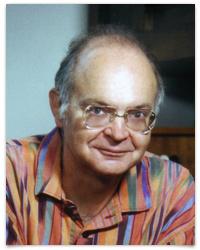
\includegraphics[scale=.5]{images/don_knuth.jpg}
\end{center}
	\caption{Don Knuth, the inventor of \TeX}
	\label{fig:sample}
\end{figure}

\section{Basic Terminology}
As usual the very basic terminology is briefly explained here. Most probably the explanations here only scratch a surface level. More detailed explanations of terminology goes into chapter~\ref{cha:theoretical-background}.

\section{Related Work and Projects}
Here a survey of other work in and around the area of the thesis is given. The reader shall see that the authors of the thesis know their field well and understand the developments there. Furthermore here is a good place to show what relevance the thesis in its field has.

\section{Structure of the Thesis}
%dsflkjas flaksjfl asdfj as lfjldsajflaksdjf sa dfjlasdkfj sadlfjasdklf als dfj l dfsdfsdfn chapter~\ref{cha:used-technologies} (\nameref{cha:used-technologies}) on page~\pageref{cha:used-technologies} we describe the used technologies.
Finally the reader is given a brief description what (s)he can expect in the thesis. Each chapter is introduced with a paragraph roughly describing its content.
\chapter{Summary}
Here you give a summary of your results and experiences. You can add also some design alternatives you considered, but kicked out later. Furthermore you might have some ideas how to drive the work you accomplished in further directions.


\chapter{Verwendete Technologien}\label{cha:used-technologies}

\setcounter{tocdepth}{4}
\setcounter{secnumdepth}{4}
\newcounter{subsubparagraph}[subsubparagraph]
\section{Unity (DM)}

\includegraphics{images/unityLogo.png} \cite{noauthor_unitylogo_nodate}
\newline
Unity ist eine Entwicklungsumgebung hauptsächlich gedacht für die Spieleentwicklung. Eigentümer des Produkts ist Unity Technologies, die ihren Sitz in San Francisco haben. 
Das Unternehmen ist seit 2004 in Betrieb und arbeitet ausschließlich an Unity und dessen Services. Die wichtigsten Services hierbei sind Unity Multiplayer, Remote Settings, der Unity Asset Store und Unity Collaborate. 

\subsection{Unity Multiplayer}
Unity Multiplayer soll es Entwicklern ermöglichen leicht und schnell, auf Mehrspieler basierende, Spiele zu entwickeln. Der Service bietet Support für die Synchronisierung von Objektpositionen zwischen den Geräten, Serverseitige Commands, die Cheating deutlich erschweren, eine Unterscheidung zwischen Client und Server im Code, sodass Entwickler auch für Einzelspieler gedachte Projekte leicht umbauen können, und vieles mehr. Der wohl größte Vorteil ist die Inkludierung eines Lobbysystems. Spieler können Lobbys erstellen und diese für andere Spieler freischalten, sodass diese der Gruppe beitreten können. Immer mehr Mehrspielerspiele, wie „Battlefield“, „Counterstrike“ oder „Destiny“, benutzen Matchmaking um Spieler, die in derselben Region spielen, in Lobbys zusammenzuschließen, um sie zu füllen. Die Spieleindustrie geht immer mehr in die Richtung, der Servicespiele. Der Grund ist, dass Spiele immer teurer werden und große Publisher nicht mehr mit den 60 Euro pro Spiel auskommen. Sie versuchen die Spiele weiter zu monetarisieren, indem sie Spielinhalte ohne zusätzliche Kosten erst spät oder gar nicht erreichbar machen. Je langlebiger die Spiele sind, desto eher ist die Wahrscheinlichkeit, dass Spieler bereit sind mehr dafür zu zahlen. Erreicht wird diese Langlebigkeit durch periodische Updates und nicht zu Letzt durch Mehrspielermodi. Spiele wie „The Division“, „Destiny“ oder „Anthem“ werden in vergleichbar schlechten Zustand veröffentlicht, mit einer großen Karte zum Erkunden und einem Mehrspielermodus. Während der nächsten Jahre werden Bugs behoben und Inhalte hinzugefügt um Spieler zurück zu bringen. Dieser Trend ist in der jetzigen Form zwar nicht wünschenswert, es ist jedoch trotzdem wichtig, dass Entwickler die Möglichkeit dazu haben. 

\subsection{Remote Settings}
Viele Mehrspielerspiele, wie „First-Person-Shooter“, MOBAs oder MMOs, benötigen regelmäßige Patches, um die Spielbalance zu verändern. Dieses Thema ist enorm komplex, da viele Räder ineinander greifen. „League of Legends“ ist seit über 10 Jahren, mit über 200 Millionen registrierten Nutzern, aktiv. Unabhängig davon wird alle 14 Tage ein Patch ausgerollt, der bestimmte Charaktere stärker und andere wieder schwächer macht. Diese Patches will der Service „Remote Settings“ ablösen, indem er Entwicklern die Möglichkeit gibt, bestimmte Werte mit der Cloud zu synchronisieren, sodass diese jederzeit über ein Webinterface, ohne zusätzliche Patches, geändert werden können. Patches sind somit nur mehr für Fehlerbehebungen und zusätzliche Inhalte nötig.

\subsection{Unity Asset Store}
Der Asset Store ist direkt in die Engine eingebaut und ist somit ein zentraler Aspekt von Unity. Er ist vor allem für Prototypen enorm wichtig und hilft Entwicklern schnell ihre Ideen zu testen und verbessern. Im Store können Nutzer Scripts, Modelle, Animationen, Tools und vieles mehr hochladen und auch herunterladen. Eine simple, aber effektive Review-Implementation ist vorhanden um hochwertige Assets zu präferieren. Inhalte sind für fast jedes Szenario und jede Idee vorhanden und deren Preise reichen von kostenlos bis zu mehr als 100 Euro. Es sind viele Modellpakete vorhanden, die oft gratis sind und für die Prototypenphase, als Platzhalter, verwendet werden. Viele Entwickler laden auch selbst entwickelte Tools, für die Kameraführung oder die Terraingestaltung, hoch. 2017 sparten Entwickler über 1 Milliarde Dollar durch die Benutzung von Assets aus dem Store.
Der Store ist aber auch zum Teil Schuld an der schlechten Reputation, die Unity, seit einiger Zeit, plagt. Unzählige Spiele werden täglich in die mobilen App Stores hochgeladen, die nur aus Asset Store Inhalten bestehen, um billige Kopien bekannter Spiele zu machen. Auch ein Grund ist, die Verwendung der Marke Unity selbst. Unity bietet eine Gratisversion, dessen größte Unterscheidung die Inkludierung des Unity Logos, am Start des Spiels, ist. Bei Bezahlversionen hat man die Wahl und da die Erscheinung des Logos meist für billige Spiele steht, entschließen sich die meisten dagegen. Die Zeit des Hochfahrens wird bei Spielen meist für die zur Schau Stellung der Technologien verwendet und die Gameengines in Verwendung entwerfen oft angepasste Logos für wichtige Spieleveröffentlichungen. Unity ist die meist verwendetste Engine am Markt und auch die erste Wahl für viele Indie Entwickler. Spiele, wie „Ori and the Blind“, „Cuphead“, „Superhot“, „Hollow Knight“, „Subnautica“ oder „Overcooked“, sind eine der größten Indie Erfolgsgeschichten in den letzten Jahren aber auch Smartphone Klassiker, wie „Angry Birds“, „Temple Run“, „Crossy Road“ oder „Pokemon Go“ sind mit Unity entwickelt worden. Jedoch erscheint das Unity Logo kaum bei Spielstart, weswegen man diese Spiele nicht sofort damit in Verbindung bringt.

\subsection{Unity Collaborate}
Unity Collaborate ist Unitys in die Engine eingebaute Git Alternative, die ein einfaches Zusammenarbeiten ermöglichen soll. Es gibt gewisse Einschränkungen, die unter gewissen Bedingungen KO-Kriterien sein können. Für Teams bis vier Personen ist der Dienst zwar gratis, werden Accounts jedoch auch mehreren Geräten genutzt, kann es zu Fehlern kommen, die behoben werden können, sofern man sich für eine der Bezahloptionen entscheidet. Unity Collaborate ist ein simples Tool, jedoch ist das neben der größten Stärke auch eine nicht zu vernachlässigende Schwäche. Ohne Erweiterungen kann der Dienst keine Dateiinhalte lesen und so Dateien zusammenfügen, wie es Git zum Beispiel kann. Es kann nur Unterscheiden in geändert oder eben nicht. Je nach Workflow kann das zum Problem werden. Ist eine strikte Arbeitsteilung vorhanden, so reicht diese Implementierung aus und macht den Dienst, so zur idealen Wahl. Arbeiten oft mehrere Leute an der selben Datei, so kann man Erweiterungen einbauen, die zusätzliche Funktionalität bieten können. Leider bietet Unity keine solchen Erweiterungen und man ist auf Dritte angewiesen.

\subsection{Unity Preispolitik \cite{noauthor_unityprice_nodate}}
Unity bietet hier drei Optionen, die sich abhängig von der Teamgröße, im Preis ändern können. Für Einsteiger und Solo Entwickler ist die Gratis Version von Unity ausreichend. Man ist in keiner Weise in den Plattformen, für die Spiele entwickelt werden können, eingeschränkt und auch der Großteil der Services ist gratis verfügbar. Support wird von Unity nicht bereit gestellt. Um diesen in eingeschränkter Form genießen zu können, wird die, 25 Dollar pro Monat kostende, Plus Version benötigt. Zusätzlicher Cloud Speicherplatz und Zugang zu einem Übungskurs sind zusätzliche Boni. Um sowohl einen „Dark Mode“, als auch ein T-Shirt zu bekommen, benötigt man die, 125 Dollar kostende, Pro Version, die alle Features, wie 20 Prozent Rabatt auf Premium Assets, mehr Cloud Speicherplatz, Zugang zu Entwicklerkonferenzen und vieles mehr freischaltet. Für größere Teams bietet Unity individuelle Lösungen. Selbst wenn man die zusätzlichen Features der Bezahlversionen nicht benötigt, ist man ab einem gewissen Umsatz dazu verplichtet.

\subsection{Plattformen}
Unity unterstützt seit vielen Jahren alle neuen Plattformen, selbst wenn diese selbst noch in Entwicklung sind. Neben den Standardplattformen, wie X-Box, Playstation, Nintendo Switch, Android, Ios, Windows, Linux und Mac werden auch Fernseherbetriebssysteme, wie Samsungs Tizen OS, Apples tvOS oder Googles Android TV unterstützt. Plattformen der Zukunft wie Microsoft Mixed Reality, Gear VR, Google Cardboard, AR-Core und viele mehr, die sich auf Augmented Reality oder Virtual Reality fokussieren, werden zahlreich unterstützt, weshalb Unity hier eine Marktdominanz zeigt. Spiele werden meist für mehrere Plattformen veröffentlicht und ein Vorteil, den Unity bietet, ist es, die selbe Codebasis für alle Plattformen zu verwenden. Ludimus hat sowohl einen Android, als auch einen Windows Client, dennoch können beide Plattformen mit dem selben Code funktionieren. Muss oder soll es jedoch Unterscheidungen zwischen Plattformen geben, so bietet Unity auch hier eine Lösung. Plattformspezifischer Code wird für alle nicht relevanten Plattformen, aus dem Code heraus geschnitten. Häufige Anwendungen hierfür sind Filesysteme und deren verschiedene Pfade. 

\subsection{Mobile Entwicklung}
Neben der Virtual und der Augmented Reality, ist Unitys Hauptverwendungszweck die mobile Entwicklung für Ios und Android. Der Vorteil der gleichen Codebasis ist hier enorm wichtig, da diese zwei Systeme sehr unterschiedliche Entwicklungsworkflows haben und es nicht effizient ist, für mehrere Plattformen einzeln zu entwickeln. Selbst große Publisher wie Square Enix, greifen bei ihrem „Tomb Raider“ Smartphone Ableger auf Unity zurück, da sie laut eigener Angabe schnell einen vorzeigbaren Prototypen bauen konnten. Auch Blizzard benutzte Unity zur Entwicklung von ihrem Kartenspiel „Hearthstone“, welches sowohl einen Android und Ios, als auch einen Windows Client, besitzt und auch sie erwähnen die schnelle Entwicklungszeit. Es sind Erfolgsgeschichten, wie diese weswegen Unity unter Entwicklern einen sehr guten Ruf genießt, auch wenn die Öffentlichkeit davon nichts mitbekommt. 

\subsection{Community}
Durch den großen Erfolg bildete sich schon zu Beginn eine riesige Community, die durch Tutorials und Livestreams von Unity selbst inspiriert wurde. Hunderte hochqualifizierte Entwickler teilen deren Wissen mit Anfängern und helfen ihnen auf ihrem Weg zum ersten Erfolg. Die Tutorials reichen von Programmierkursen, über die Modellierung, bis hin zur Integration anderer Dienste in Unity. Die Gemeinschaft ist groß genug, sodass jedes gewünschte Verhalten dokumentiert worden ist, oder jeder aufgetretene Fehler behoben worden ist.

\subsection{Integration}
Unity bietet Integrationen mit vielen Modellierungs-, Zeichen- und Audiotools. Die zwei am meisten vorkommenden Kombinationen sind wohl: Unity und Blender und Unity und Photoshop.
\subsubsection{Unity und Blender} \label{sec:unity-blender}
Blender ist eine gratis Open Source Modellierungssoftware, die in viele Formate exportieren kann und auch eine ähnliche Community, wie Unity, bietet. In vielen Tutorials werden Unity und Blender gemeinsam verwendet, da beide Programme zwar Einsteigerfreundlich sind, jedoch auch enormes Potenzial haben, sofern gebraucht. 
\subsubsection{Unity und Photoshop}
Für die 2D Spieleentwicklung sind Sprites, also Bilder, enorm wichtig. Viele Guides empfehlen hier meist Photoshop, den sowohl verschiedene Layer als auch Animationen werden perfekt unterstützt, um einen reibungslosen Workflow zu garantieren.

\section{Entwicklung mit Unity (DM)}
Die Entwicklung in Unity ist in viele kleine Bereiche aufgeteilt. Logik implementiert man jedoch immer in C-Sharp, sofern man keine explizite Lizenz für C++ erworben hat. Im Laufe des Jahres 2019, soll jedoch eine Visual Scripting Lösung getestet werden. Visual Scripting ist eine Drag and Drop Art der Programmierung. Ein Programm besteht hier aus Nodes. Diese Nodes haben bestimmte Funktionen, die miteinander verbunden werden können. Entwickler können eigene Nodes schreiben, um die Grundfunktionalität zu erweitern. Das bekannteste Beispiel dieser Entwicklungsmethode ist die Unreal Engine 4, die dieses Konzept schon seit Beginn nutzt. 
\subsection{Editor}
\begin{figure}
    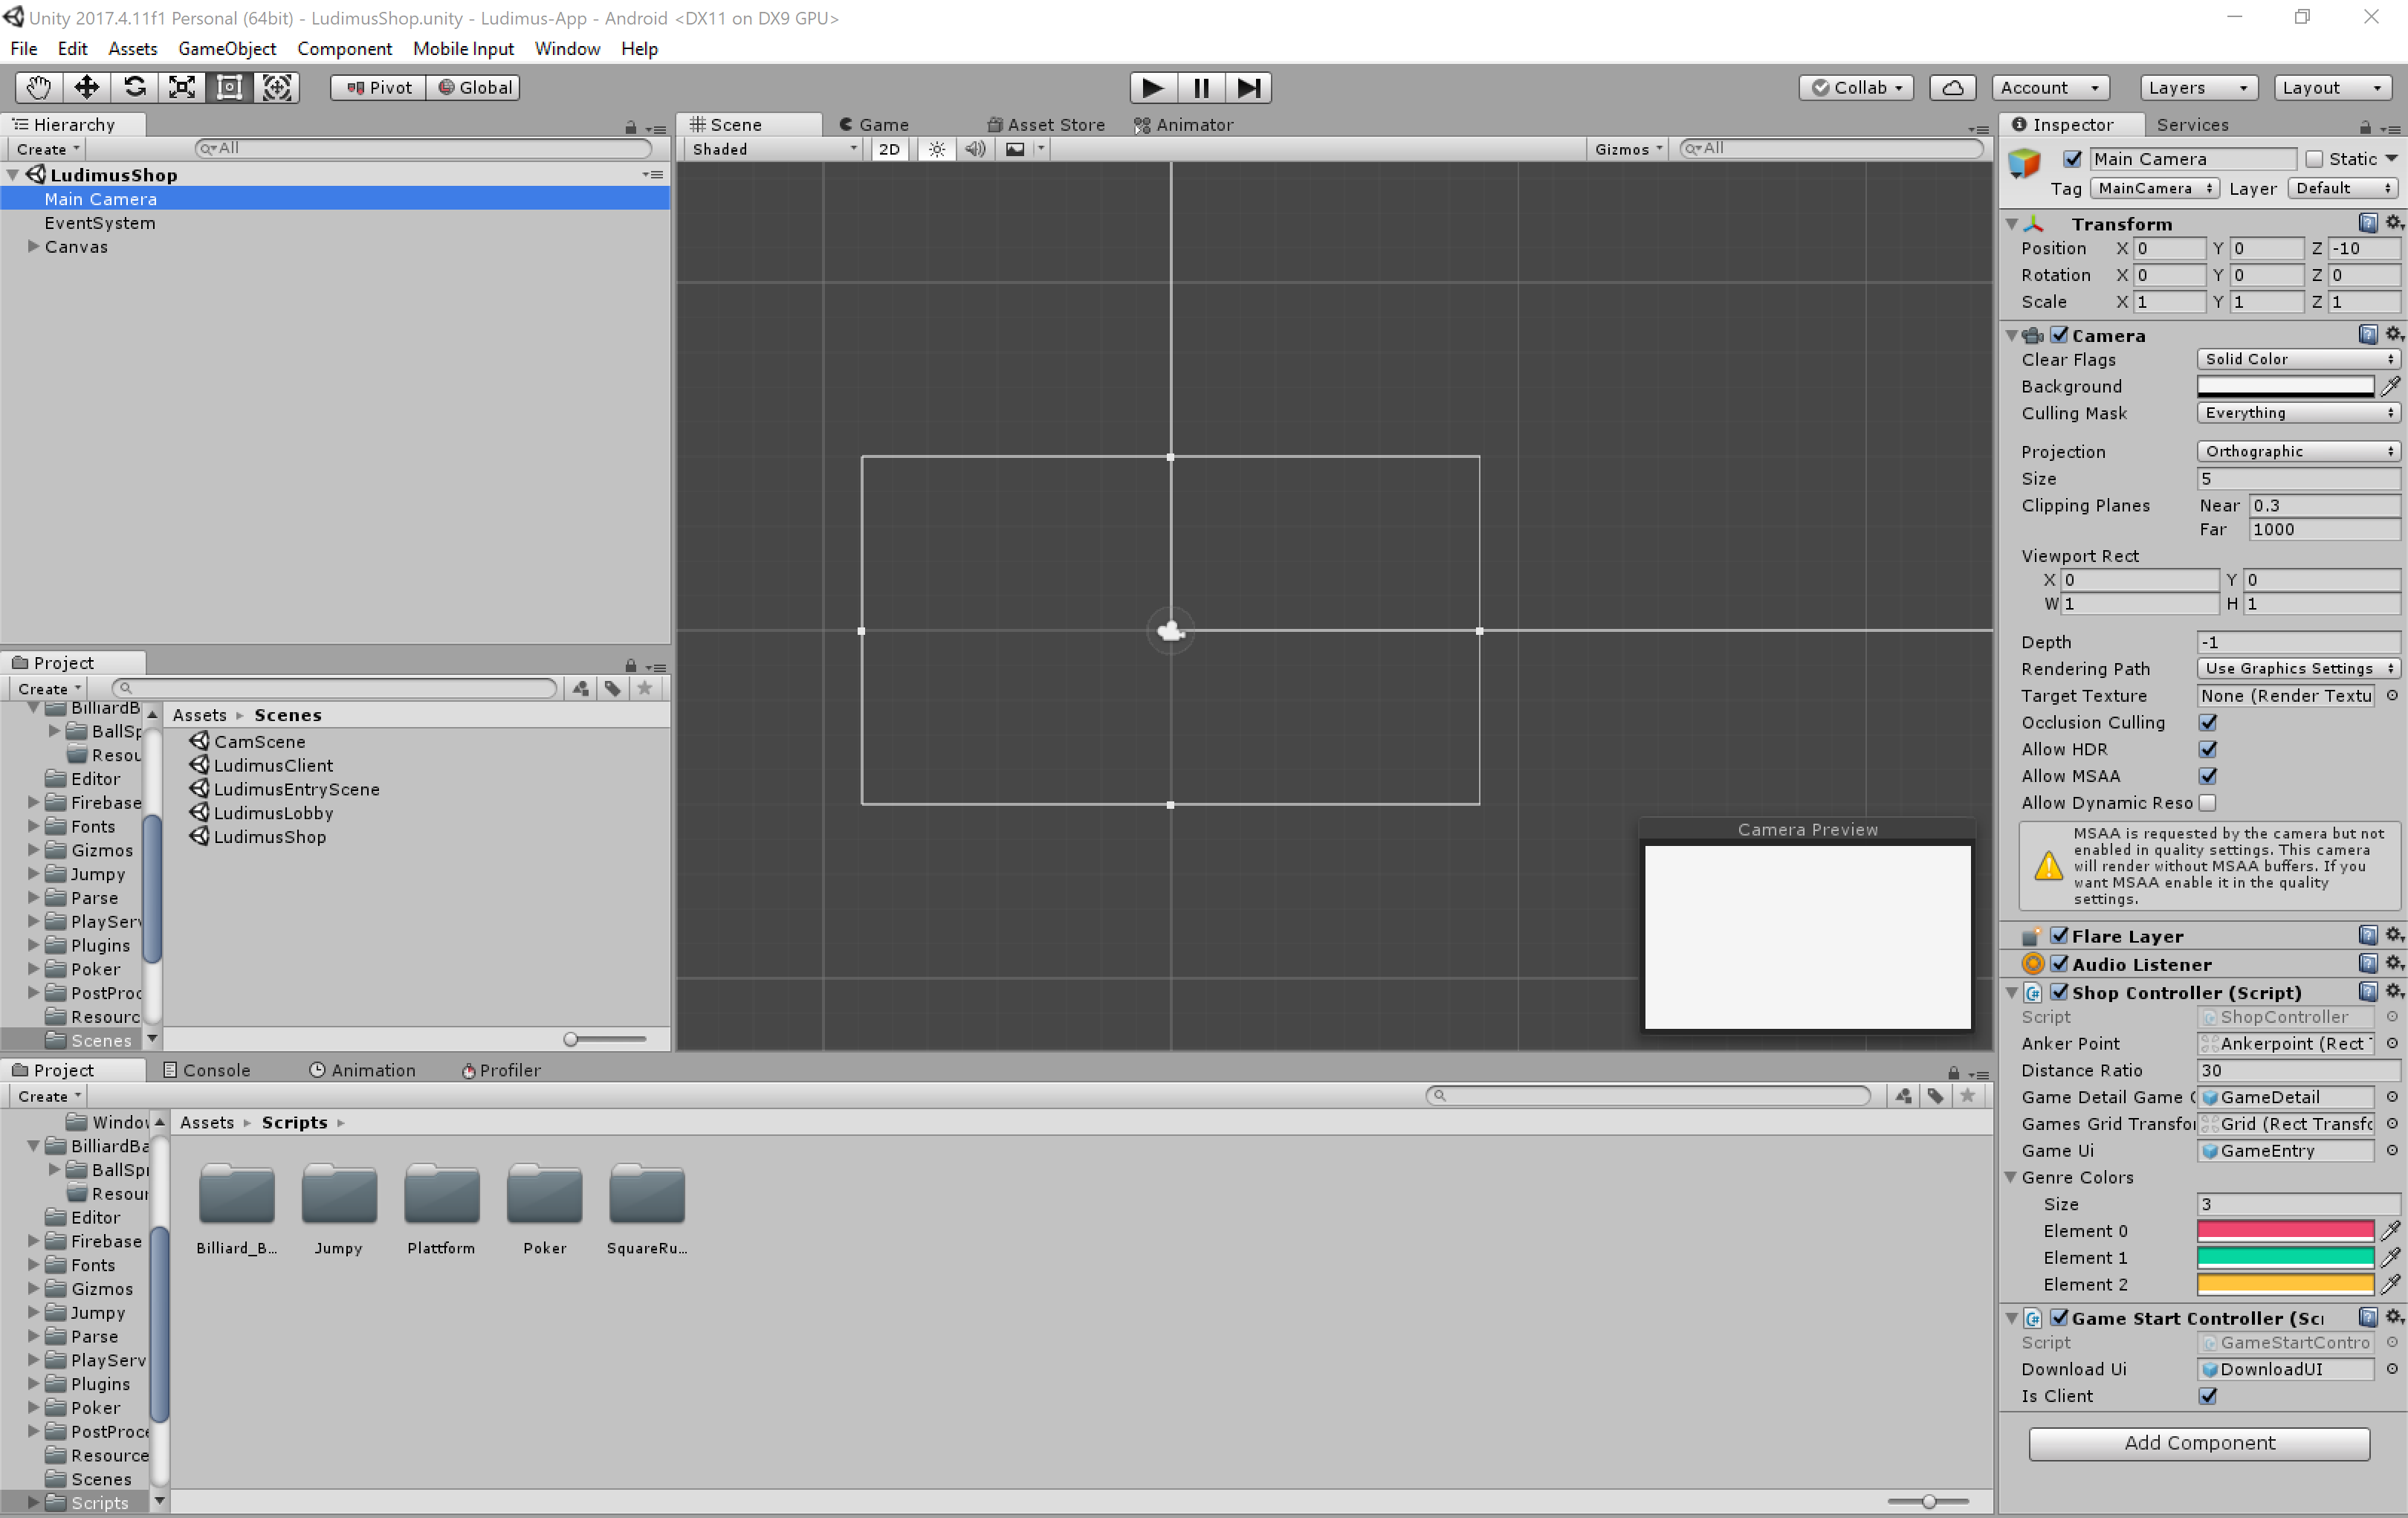
\includegraphics[scale=0.35]{images/unityEditor.png} 
    \caption{Unity Editor}
    \label{img:unity-editor}
\end{figure}

Der Editor ist in Tabs gegliedert, wie in Abbildung \ref{img:unity-editor} zu sehen, die beliebig angeordnet werden können. Wichtige Tabs sind:
\subsubsection{Hierarchy}
Hier werden alle Objekte, die in der aktuell ausgewählten Szene sind, angezeigt. Objekte können verschachtelt sein oder unabhängig voneinander herumverschoben werden. Die Details der ausgewählten Elemente werden im Inspector angezeigt.
\subsubsection{Scene}
Das Scene Fenster zeigt die Welt, die aktuell ausgewählte Szene, in der die Objekte existieren. Alle Objekte haben eine eindeutige Position, mit einer x, y und z Koordinate. Der Benutzer kann sich in diesem Dreidimensionalen Raum frei bewegen und Objekte anordnen, um seine Level zu gestalten. Da Unity sowohl 2D als auch 3D Entwicklung unterstützt, kann man die Perspektive einstellen.
\subsubsection{Project}
Der Project Tab die In Engine Version des Fileexplorers. Er verfügt über eine schnellere Suchfunktion und ein Favoritensystem. Hier ausgewählte Objekte können sowohl in die aktuelle Szene hineingezogen werden oder die Details, im Inspector, angesehen werden.
\subsubsection{Console}
Die Konsole zeigt alle Konsolen Einträge auf, gruppiert nach Art, sprich „log“, „warning“ oder „error“. Wählt man einen Eintrag aus, so sieht man dessen Details und kann auch zur Zeile im Code springen, der diesen ausgelöst hat. Die Standard Lösung von Unity verfügt über keine Suchfunktion, jedoch gibt es Tools im Asset Store, die diese Lücke füllen.
\subsubsection{Animation}
Soll sein Spiel über bewegliche Inhalte verfügen, so sind Animationen oft eine gute Lösung. Unity verwendet hier das Keyframe Prinzip, bei dem alle Eigenschaften zu zwei bestimmten Zeitpunkten, Keyframes, gespeichert werden, und anschließend alle Änderungen über die Zeit verteilt durch geführt werden. Unity unterstützt diese Art der Animation für 3D-Modelle, Sprites und UI-Elemente. 3D-Modelle und Sprites können mit einem Skelett versehen werden, dass bewegt werden kann um auch das Modell selbst zu bewegen.
\subsubsection{Game}
Ist es Zeit das Programm zu testen, so kann man es mithilfe des großen Spielen-Knopf starten. Unity wechselt danach automatisch in den Game Tab. Hier sieht man seine Szene durch eine Kamera, genauso wie sie Spieler später sehen würden. Dieser Modus ist für schnelle Testläufe ideal. Es gibt jedoch unterschiede zwischen dieser spielbaren Version und einer gebauten App, weshalb es ratsam ist, beide Versionen zu überprüfen.
\subsection{Komponenten}
Objekte in Unity bestehen aus Komponenten. Diese geben ihnen ihre Funktionalität und bieten gleichzeitig Flexibilität. Alle vom Entwickler generierten Scripts erben automatisch von der Basisklasse MonoBehaviour, wodurch sie als Komponenten verwendet werden können. Als Basis bietet Unity jedoch schon eine Reihe an Komponenten an, um Beispielsweise ein Objekt auf Gravitation reagieren zu lassen. Diese bereitgestellten Komponenten sind eingeteilt in: Mesh, Effects, Physics, Navigation, Audio, Video, Rendering, UI, AR und vielen mehr.
\subsubsection{Mesh}
Diese Gruppe besteht aus 3 verschiedenen und essentiellen Komponenten, für die 3D Entwicklung. Der Mesh Filter gibt an welches Modell dieses Objekt darstellen soll. Der Mesh Renderer hingegen beschreibt, welche Materialien das Objekt bekommt oder ob es Schatten erhalten oder werfen soll. Um 3D Text in der Szene anzuzeigen, benötigt man den Text Mesh Komponenten.
\subsubsection{Effects}
Egal ob Lagerfeuer, kleine Luftsteifen, um Bewegung deutlicher zu machen, oder Lens Flare Effekte, wenn der Spieler in die Sonne sieht, Effekte sind in Spielen häufig verwendet und Unity bietet hier eine gute Basis um seine eigenen Effekte zu erzeugen.
\subsubsection{Physics}
Dieser Punkt ist unterteilt in 2D und 3D Physics, um für Klarheit zu sorgen.
\paragraph{2D Physics}
Um die vorher erwähnte Gravitation für dieses Objekt zu aktivieren, benötigt man einen Rigidbody, hier konkret Rigidbody2D. Unity bietet eine globale Vektor Variable für die Gravitation, mit einer x und einer y Richtung. Im Rigidbody kann man die Stärke des Effekts auf dieses eine Objekt verändern. Die Werte für Masse, Trägheit und verschiedene Physics Materialien können eingetragen werden. Letztere bestimmen, wie stark das Objekt von Reibung beeinflusst wird und wie federnd es ist. Objekte können auch in ihrer Bewegung oder Rotation für verschiedene Achsen eingeschränkt werden.
Zusätzlich zum Rigidbody findet man hier alle Arten von Collidern, die Unity für 2D zu bieten hat. Diese Collider beschreiben die Zone, in der Kollisionen registriert werden. Collider können miteinander verknüpft werden, um die Objekte perfekt einzuhüllen. Box-, Circle-, Edge- und Polygon-Collider sind die am häufigsten verwendeten. Während Box- und Circle-Collider nur geometrische Formen beschreiben und lediglich in deren Größe geändert werden können, bieten sowohl Edge-, als auch Polygon-Collider Möglichkeiten, die für 3D nicht denkbar sind. Edge-Collider werden oft für Plattformen verwendet, da sie nur eine Linie darstellen, die an verschiedenen Punkten abgebogen werden kann. Das selbe Prinzip verfolgt der Polygon-Collider, nur verbindet er Start- und Endpunkt miteinander. Hinzukommt eine automatische Erkennung, der Form, bei Sprites. 
Als dritte Gruppe dieser Kategorie gelten die Joints. In verschiedenen Ausführung regeln sie das Verhalten zwischen zwei Objekten. Räder, Dämpfungen, Seile und mehr können so realisiert werden.
Zu guter Letzt gibt es noch Effectors. Diese regeln die Bewegungen, wenn zwei Objekte miteinander kollidieren. So können „One-Way“ Plattformen oder Förderbänder geschaffen werden.
\paragraph{3D Physics}
Die Rigidbody Implementierung für den dreidimensionalen Raum stellt eine abgespeckte Version, im Vergleich zur 2D, dar. Hier kann die Gravitation nur ein- oder ausgeschaltet werden und keine Physics Materialien zugeteilt werden.
Bei den Collidern finden sich Implementierungen der Standard Formen, wie Würfel oder Kreis ,wieder, hinzugekommen sind jedoch der Mesh Collider, der eine ähnliche Funktionsweise, wie der Polygon-Collider, darstellt und der Wheel Collider, der detaillierte Entscheidungsmöglichkeiten bezüglich Reifendruck, Federung, Reibung, in verschiedene Richtungen, und vielen mehr, bietet. 
Auch Effectors werden hier wieder aufgelistet, jedoch ist sticht die Cloth Komponente hier heraus. Sie ermöglich es Kleidung zu simulieren, um zum Beispiel im Wind zu flattern.
\subsubsection{Navigation}
Navigation ist nur für 3d Projekte verwendbar und ermöglicht es Entwicklern für jeder Objekt einzustellen, ob es begehbar ist, um anschließend Gegnerobjekten, oder anderen Objekten, die Wegfindung benötigen, einen sogenannten Nav Mesh Agent zu geben. Dieser Agent enthält Werte für Höhe, die maximale Schräge, die er bezwingen kann, und die maximale Stufenhöhe. Der Entwickler muss nur noch ein Ziel übergeben und das Objekt kann sich selbstständig dorthin bewegen.
\subsubsection{Audio}
Hier können Entwickler Objekte mit Fähigkeiten für das Zuhören oder das Sprechen ausstatten. Bestimmte Audiofilter für Echoeffekte können auch erstellt werden.
\subsubsection{Video}
Als einziges Element in dieser Gruppe, ist der Video Player das Werkzeug zum Präsentieren von vorher gerenderten Zwischenszenen.
\subsubsection{Rendering}
In jedem Spiel wird eine virtuelle Kamera verwendet, durch deren Linse gespielt wird. Diese Kamera Komponente ist unter dem Begriff Rendering, mit einer Skybox-, einer Licht- und der Sprite Renderer Komponente zu finden.
\paragraph{Camera}
Hier können wichtige Einstellung bezüglich der Darstellung getroffen werden. Von oben beginnend, kann der Entwickler gleich den Hintergrund festlegen. Standardmäßig ist er blau. Neben Farben können Entwickler jedoch auch Skyboxen auswählen. Mit der Option der Culling Mask, können bestimmte Schichten aktiviert oder deaktiviert werden. Die Projektion beschreibt die Art, wie mit entfernten Objekten umgegangen werden soll. Während Perspective Objekte, die in der Ferne liegen kleiner darstellt und so für 3D Spiel ideal ist, behält Orthograpfic die Originalgröße der Objekte unabhängig von deren Entfernung zu Kamera bei und eignet sich somit für 2D Spiele. Abhängig davon kann der Entwickler das Field of View oder die Kameragröße einstellen. Um zu verändern wie nah oder fern Objekte von der Kamera entfernt sein dürfen um gesehen zu werden, dient die Clipping Planes Option. Die restlichen Optionen sind für verschiedene Rendering Arten oder ob das gerenderte Bild gespeichert werden soll, um eine Karte zu erzeugen.
\paragraph{Skybox}
Die Skybox Komponente wird verwendet, um einen Himmel zu simulieren. Dazu benötigt man ein Skybox Material, welches dann hier verwendet werden kann.
\paragraph{Light}
Die Licht Komponente wird verwendet um Sonnenlicht, Licht von Lampen, Lagerfeuer und mehr zu simulieren. Dieses breite Aufgabengebiet wird mittels Untertypen realisiert.
\subparagraph{PointLight}
Punktlichter erleuchten einen bestimmten Bereich von einem Punkt aus in alle Richtungen. Lagerfeuer oder Lampen sind hier die Einsatzzwecke.
\subparagraph{Arealight}
Licht wird von einem bestimmten Punkt in einer Kegelform, in eine Richtung, versendet. Diese Methode ist für Scheinwerfer oder Spezielle Straßenlaternen sehr nützlich.
\subparagraph{Directionlight}
Um die Sonne zu simulieren, werden direktionale Lichter verwendet. Diese werfen Licht von überall in eine bestimmte Richtung, weshalb die Position keine Rolle spielt. 
\paragraph{Sprite Renderer}
Diese Komponente ermöglicht es Sprites in der Welt anzuzeigen. Das ausgewählte Sprite kann in der Farbe im Editor geändert werden, weshalb Sprites oft in Grautönen eingelesen werden, um sie in der Engine anzupassen, durch die Änderung des Order Layer vor oder hinter anderen Sprites angezeigt werden oder durch Materialen bestimmte Effekte, wie Wasserreflexionen, erhalten.
\subsubsection{UI}
Alle Komponenten, die mit der Erstellung eines Userinterfaces zusammen hängen, sind hier untergebracht. Es sind Presets für Buttons, Dropdown Menüs, Eingabefelder und vieles mehr vorhanden. UI-Elemente werden wie normale Objekte im dreidimensionalen Raum gesehen, weshalb Elemente auch nicht mit Code, wie html oder css, erzeugt und verändert werden können. 
\subsubsection{AR}
Je nach Plattform ändert sich die Größe dieses Menüs. SDKs für Geräte ähnlich der HoloLens bieten hier Komponenten für Spatial Recognition und mehr. 
\subsection{Scripts}
Diese Komponenten bieten ein solider Grundkonstrukt. Um Funktionalität in ein Spiel zu bringen werden jedoch, eigens geschriebene, Scripts benötigt, die wie folgt aufgebaut sind.
Wie bereits erwähnt, erben diese Programmteile von der Basisklasse MonoBehaviour. Lässt man sich die Scripts in der Engine generieren, so erhält man ein File ähnlich dem in Abbildung \ref{img:unity-basescript}.
\begin{figure}
    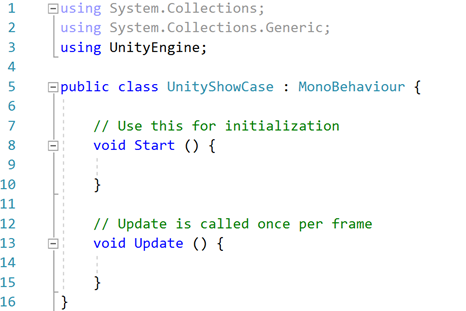
\includegraphics[scale=0.8]{images/unityScriptBase.png}
    \caption{Unity Basisscript}
    \label{img:unity-basescript}
\end{figure}
\subsubsection{Lifecycle Methoden}
Für Einsteiger sind die zwei generierten Methoden, Start und Update, kommentiert. Unity bietet verschiedene Lifecycle Methoden, die unterschiedliche Zwecke und Anwendungsbereiche haben, an.
\paragraph{Awake}
Die erste Methode, die für jedes Objekt aufgerufen wird ist Awake. Hier soll Code ausgeführt werden, der nur einmal ausgeführt werden darf.
\paragraph{OnEnable}
Objekte in Unity können jederzeit aktiviert oder deaktiviert werden. Werden Objekte aktiviert wird diese Methode aufgerufen. Diese Methode kann genutzt werden um andere Objekte auch zu aktivieren.
\paragraph{Start}
Start wird immer nach OnEnable aufgerufen und wird primär für die Verknüpfung zwischen Komponenten benutzt.
\paragraph{FixedUpdate}
Unity unterscheidet in zwei verschiedene Updatemethoden. FixedUpdate wird, wie der Name vermuten lässt, immer in selben Zeitintervallen aufgerufen, während Update immer dann verwendet wird, sobald ein neues Bild erschienen ist. FixedUpdate wird für Physikberechnungen und Eingabeüberprüfungen verwendet, die zwischengespeichert werden um in der Update Methode verwendet zu werden.
\paragraph{Update}
Hier wird die Logik des Spiels behandelt. Sollen Objekte bewegt werden, soll dies mit den vorher eingelesenen Werten hier geschehen. Haben bestimmte Aktivitäten eine Abklingzeit, bevor sie wieder verwendet werden können, so werden die Überprüfungen hier durchgeführt.
\paragraph{LateUpdate}
Wird für Kamerabewegungen genutzt und wird nach allen anderen Updates aufgerufen.
Anschließend wird das aktuelle Bild erzeugt und der Kreislauf beginnt bei FixedUpdate erneut.
\paragraph{OnDisable}
Wird ein Objekt während dieses Bildes deaktiviert, so wird diese Methode verwendet um zu reagieren. 
\paragraph{OnDestroy}
Wird dieses Objekt zerstört, zum Bespiel sobald der Spieler verloren hat, so dient diese Methode um den Score zu speichern oder ein bestimmtes UI aufzurufen.
\subsubsection{Kollisionen}
Kollisionen passieren, wenn zwei Collider desselben Typs, sprich 2D mit 2D und 3D mit 3D, miteinander kollidieren. Abhängig von deren Eigenschaften werden verschiedene Events aufgerufen.
\paragraph{OnCollisionEnter}
Kollidiert ein Collider mit einem anderen und beide haben die Standardeinstellungen ausgewählt, so wird diese Methode während dem Bild der Berührung aufgerufen.
\paragraph{OnCollisionEnter2D}
Ist das 2D Abbild der oben beschriebenen Methode.
\paragraph{OnCollisionStay/OnCollisionStay2D}
Solange zwei Collider miteinander kollidieren, wird diese Methode benutzt.
\paragraph{OnCollisionExit/OnCollisionExt2D}
Trennen sich die zwei Objekte nun wieder, kommt diese Methode zum Einsatz.
\subsubsection{Trigger}
Jeder Collider hat die Option ein Trigger zu sein oder nicht. Trigger registrieren zwar auf Kollisionen im Code, prallen jedoch nicht voneinander ab. Kollidiert ein Objekt, welches einen Collider mit einem aktiven Trigger hat, mit einem anderen Objekt, unabhängig von dessen Optionen, so werden folgende Events stattdessen ausgeführt.
\begin{description}
    \item OnTriggerEnter/OnTriggerEnter2D
    \item OnTriggerStay/OnTriggerStay2D
    \item OnTriggerExit/OnTriggerExit2D
\end{description}
\subsubsection{Objekte erzeugen}
Im Editor können Objekte mit Drag and Drop in die Szene hineingebracht werden. Will man jedoch zur Laufzeit Objekte erzeugen, so funktioniert dieser Ansatz nicht. Die Methode Instantiate erledigt dies, es gibt jedoch verschiedene Möglichkeiten diese zu benutzen.  Durch die letzten Parameter kann eingestellt werden, wo und als Kind welchen Elements das Objekt erzeugt wird. Im ersten Parameter muss man das Objekt selbst angeben, wobei der Entwickler hier 3 Optionen hat.
\paragraph{Resources}
Bestimmte Ordnernamen sind mit speziellen Funktionen belegt. Der StreamingAssets Ordner zum Bespiel ist für nicht zu kompilierende Inhalte bereitgestellt. Um Objekte einfach zu erzeugen, dient der Resources Ordner. Gespeicherte Objekte können aus diesem über ihren Name erzeugt werden mit der Zeile aus Abbildung \ref{img:unity-instantiate01}.
\begin{figure}
    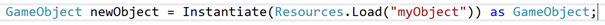
\includegraphics[scale=0.8]{images/unityInstantiate01.png}
    \caption{Objekt erzeugen über Resources}
    \label{img:unity-instantiate01}
\end{figure}
\begin{figure}
    
\includegraphics[scale=0.8]{images/unityInstantiate02.png}
    \caption{Objekt erzeugen durch Klonen eines Objektes}
    \label{img:unity-instantiate02}
\end{figure}
\paragraph{Klonen}
Um Objekte schnell klonen zu können, dient die Zeile aus \ref{img:unity-instantiate02}.

\paragraph{Referenzen}
Die selbe Syntax, jedoch einen anderen Verwendungszweck hat die Erstellung von Objekten mittels Referenzen. Ein Objekt kann als öffentliche Variable gespeichert werden, um später eine Instanz davon zu erstellen.
\subsubsection{Öffentliche Variable und Verlinkung zwischen Komponenten}
Unity bietet mehrere Möglichkeiten für die Erstellung von Referenzen zwischen Komponenten, wobei deren Einsatz sich deutlich unterscheidet.
Um auf Komponenten eines Objektes zugreifen zu können, benötigt man zuerst eine Referenz auf dieses Objekt selbst. Die Methode GetComponent() gibt anschließend den gewünschten Komponenten zurück. Referenzen auf Objekte kann man durch Filtern aller Objekte bekommen, zusehen in Abbildung \ref{img:unity-getallobjects}.
\begin{figure}
    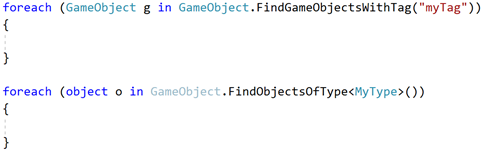
\includegraphics[scale=0.8]{images/unityGetAllObjects.png}
    \caption{Beschaffung aller Objekte mit einer bestimmten Eigenschaft}
    \label{img:unity-getallobjects}
\end{figure}
Objekte werden meist mit Tags versehen, weshalb die erste Methode öfter verwendet wird. Will man jedoch nur ein bestimmtes Objekt, so ist es nicht ratsam alle Objekte auf deren Namen zu überprüfen. Hier bietet Unity ein extrem brauchbares Features, welches bei öffentlichen Variablen Standard ist, jedoch mit der Annotation SerializeField auch für private Felder verwendet werden kann, siehe Abbildungen \ref{img:unity-serializefield} und \ref{img:unity-puplicfield}. Die Werte dieser Felder können über den Inspector gesetzt werden, wie in \ref{img:unity-inspectorsimple} und \ref{img:unity-inspectoradvanced} zu sehen.
\begin{figure}
    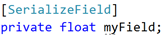
\includegraphics[scale=0.8]{images/unitySerializeField.png}
    \caption{Privates Feld mit SerializeField Annotation}
    \label{img:unity-serializefield}
\end{figure}
\begin{figure}
    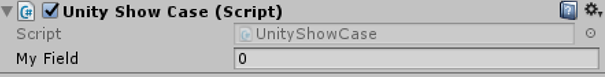
\includegraphics[scale=0.8]{images/unityInspectorSimple.png}
    \caption{Inspector Ansicht von Feldern}
    \label{img:unity-inspectorsimple}
\end{figure}

Erstellt man öffentliche Felder mit den Komponenten oder einem Objekt als Typ, wie in Abbildung \ref{img:unity-puplicfield}, so kann man diese im Inspector per Drag and Drop belegen, zu sehen in \ref{img:unity-inspectoradvanced}.
\begin{figure}
    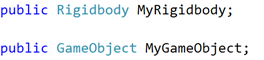
\includegraphics[scale=0.8]{images/unityPuplicField.png}
    \caption{Öffentliche Felder mit komplexen Datentypen}
    \label{img:unity-puplicfield}
\end{figure}
\begin{figure}
    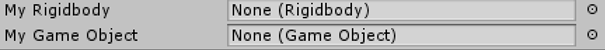
\includegraphics[scale=0.8]{images/unityInspectorAdvanced.png}
    \caption{Inspector Ansicht von mehreren komplexen Feldern}
    \label{img:unity-inspectoradvanced}
\end{figure}

Diese Methode wird verwendet, wenn Referenzen auf andere Objekte nötig sind. Den eigenen Rigidbody, sollte man jedoch nicht so referenzieren. Hier sollte eine private Variable angelegt werden, die mit GetComponent() in der Start Methode initialisiert wird, siehe Abbildung \ref{img:unity-getcomponent}.
\begin{figure}
    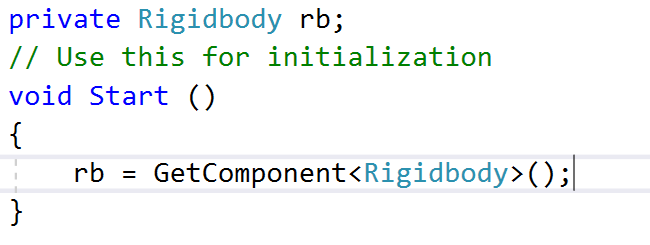
\includegraphics[scale=0.8]{images/unityGetComponent.png}
    \caption{Rigidbody des eigenen Objektes erhalten}
    \label{img:unity-getcomponent}
\end{figure}
\subsection{Alternativen}
Unity ist nicht die einzige Spieleengine und andere Optionen wie die Unreal Engine 4 oder Gamemaker Studio, wären valide Optionen gewesen. Unity bietet jedoch soliden Support für sowohl 2D als auch 3D, wodurch wir in keinster Weise eingeschränkt waren.  Den größten Vorteil der Unreal Engine, die unglaublich mächtige Rendering Pipeline, würde von unseren Spielen nie ausgereizt worden, weshalb wir uns für die Unity Game Engine entschieden, nicht zuletzt wegen unserer schon vorhandenen Erfahrung und der riesigen Community.
\section{Firebase (DM)}

\includegraphics{images/firebaseLogo.png} \cite{noauthor_firebaselogo_nodate}
\newline
Firebase ist eine einfach zu bedienende Serveralternative, die Datenbank, Fileserver, Authentifizierung, Website Hosting und mehr über ein Webinterface vereint. Im Vergleich zu regulären Servern macht es Firebase einfacher für den Entwickler, sodass dieser mehr Zeit in sein Produkt selbst investieren kann. 
Firebase bietet fortgeschrittene Sicherheitsmechanismen, Synchronisierung mehrerer Serverstandorte, Erreichbarkeit immer und überall und Offline Funktionalität.
Alle Produkte sind mit verschiedensten Anmeldeoptionen verknüpfbar, wie Google Sign-In,
Facebook Sign-In, Email/Passwort, Google Play, usw..
\subsection{Datenbank}
Firebase bietet hier zwei Möglichkeiten zur Speicherung von Daten, wobei beide auf NoSql-Datenbanken zurückgreifen. Daten können über das Webinterface angesehen, geändert und auch hinzugefügt werden.
\subsubsection{Cloud Firestore}
Diese neue Datenbanklösung ist zwar momentan noch in der Beta, ist jedoch von Beginn an für Skalierbarkeit optimiert. Wie für NoSql-Datenbanken üblich, wird enormer Fokus auf Lesegeschwindigkeiten und weniger auf Schreibgeschwindigkeiten gelegt. Verstärkt wird dieser Effekt dadurch, dass Indexe auf alle Felder gelegt werden um die gleichen Datenzugriffszeiten für 100 als auch für 100 Millionen Daten zu garantieren. Cloud Firestore bietet momentan SDKss für Android und Ios Apps, Web, Node, Java, Python und Go an. Der Service verfügt unter Android, Ios und Web über die Möglichkeit, Daten lokal zu zwischenspeichern, wenn die Verbindung einmal verloren geht und diese dann mit dem Server zu synchronisieren, sobald das Problem behoben worden ist. Cloud Firestore ist eine dokumentenbasierte Lösung, was bedeutet das Objekte als Dokumente in einer Collection gespeichert werden. Diese Art der Speicherung wird oft als semistrukturierte Datenspeicherung bezeichnet. Dokumente haben verschiedene Felder, wobei Felder wieder Collections mit Dokumenten enthalten können. Diese sogenannten Subcollections ermöglichen in der Theorie zwar ein 1:1 Abbild der Datenstruktur aus Objektorientierten Sprachen, da diese jedoch nur einzeln gequeried werden können und nicht inkludiert werden können, verursacht diese Methode nur mehr Komplikationen. Eine Realisierung mittels Arrays von Referenzen, wäre hier die einfachere Variante, da Arrays inkludiert werden und, sofern das Programm das einlesen dieser händelt, einfach geparst werden können. Dieser Aufbau ähnelt sehr einer Relationalen Datenbankstruktur.
\subsubsection{Realtime Database}
Realtime Database bietet viele der selben Vorteile, wie Cloud Firestore. Nur der Fokus auf Skalierbarkeit ist nicht so stark ausgeprägt, jedoch ist das System stabiler, da es schon länger auf dem Markt verfügbar ist. SDKs gibt es für Android, Ios, Web, C++ und Unity. Neben der besseren Verfügbarkeit der SDK für Unity war ein Mitentscheidungsgrund die Stabilität, die die Realtime Database bietet. Die Synchronisierung Offline geänderter Daten ist für Android und Ios verfügbar, nicht jedoch für Webanwendungen. Wir benutzen jedoch keine der drei Plattformen, und selbst wenn können unsere Nutzer keine Daten ändern oder einfügen, weshalb dieses Feature keine Bedeutung für uns hatte. Die Skalierbarkeit ist momentan noch kein Bedenken und der Umstieg auf Cloud Firestore ist auch während der Entwicklung noch leicht genug. Die Realtime Database benutzt die Key-Value Notation für die Datenspeicherung. Diese Schreibweise ähnelt JSON sehr, wodurch das einlesen und auslesen von Daten deutlich erleichtert wird.

Wir entschieden uns für die Realtime Database aus mehreren Gründen. Die Verfügbarkeit der SDK für Unity ist ein KO-Kriterium, da diese Technologie nicht änderbar ist und die Verwendung der Rest-Schnittstelle von Cloud Firestore außer Frage stand. Zusätzliche Features wie bessere Skalierbarkeit, bessere Offline Funktionalitäten oder strukturiertere Daten bringen wenig bis keinen Vorteil, da unsere Datenbank nur die Spiele speichert, die zur Verfügung stehen, diese keine komplexen Attribute haben, welche Referenzen benötigen würden und wir keine Offline Funktionalität brauchen. Falls die Datenbank jedoch über eine gewisse Größe hinweg wachsen würden, wäre ein Umstieg auf Cloud Firebase denkbar, da die Preispolitik diesen Usecase unterstützt.
\subsection{Storage}
Firebase bietet ein simples Filesystem, mit dem man Dateien in Ordnerstrukturen speichern kann. Von jeder Datei wird die Größe, der Typ, das Erstell- und Änderungsdatum und die Download URL angezeigt. Durch die SDKs ist die Navigation durch die Ordnerstruktur und das downloaden von Dateien unkompliziert. Als Administrator erhält man eine Übersicht über alle Downloads, die momentane Speichergröße und die momentane Anzahl an Elementen, für einen bestimmten Zeitraum. 
\subsection{Hosting}
Firebase ermöglicht es auch eine Webseite zu hosten. Eine Übersicht über alle Uploads mit deren User ist vorhanden um auch zwischen Versionen zu wechseln. Man kann seine Seite auch mit einer eigenen Domain verbinden.
\subsection{Authentifizierung}
Wie bereits erwähnt bietet Firebase hier viele Möglichkeiten für Entwickler Ihre User anzumelden. Anmeldeoptionen von etablierten Netzwerken wie Facebook, Twitter, GitHub, Google Play oder Google sind unterstützt, ebenso wie Telefonauthentifierung, Gastaccounts oder Authentifizierung über Email und Passwort. Es stehen auch Templates für Email-Adressen Bestätigung, Passwort zurücksetzen, usw. zur Verfügung. 
Im Webinterface ist eine Auflistung aller registrierten Accounts, mit deren Anmeldeoption, dem Datum der Erstellung und dem Datum des letzten Logins, ersichtlich.
Werden Telefonbestätigungen verwendet, sieht man diese als Graph dargestellt. Die Einbindung der Authentifizierung in andere Firebaseprodukte ist über sogenannte Regeln implementiert. Hier kann der Admin einstellen ob, oder wer Schreibzugriff auf die Datenbank hat. Kann jeder schreiben, der eingeloggt ist, so gibt es die globale Variable „auth“, deren Wert man mit null vergleicht. Diese Regeln können mit einem Simulator getestet werden um Fehler zu vermeiden.
\subsection{Preispolitik}
Firebase bietet drei verschiedene Modelle, wobei eines kostenlos ist und die restlichen beiden kostenpflichtig sind. 
Der „Spark Plan“ ist die gratis Version. Man hat Zugriff auf Datenbank, Fileserver, Website Hosting, Authentifizierung und den Großteil der restlichen Produkte. Jedoch sind bestimmte Nutzungsgrenzen für die verschiedenen Tätigkeiten festgelegt. Die Datenmenge der Realtime Database, darf zum Beispiel nicht über ein Gigabyte groß sein und es dürfen auch nicht über zehn Gigabyte heruntergeladen werden. Für Ludimus sind das jedoch astronomische Grenzen, die nur mit extrem vielen Spielen erreicht werden können. Unsere Anwendung verbraucht vielmehr Fileserverkapazitäten, die bei diesem Modell bei fünf Gigabyte liegen und es dürfen maximal ein Gigabyte pro Tag heruntergeladen werden. Mit genügend Nutzern sind das die ersten Schwellpunkte die überschritten werden. 
Für 25 Dollar pro Monat kann man Subscriber des „Flame Plans“ sein. Dieser hebt die Nutzungsgrenzen aller Produkte um einiges.
 Da wir diese Erhöhung jedoch nur für ein Produkt brauchen, und wir hier nicht allein sind, ist die dritte Möglichkeit, der „Blaze Plan“, „Pay as you go“, heißt man zahlt nur, was man benötigt. Zur Schätzung der Kosten bietet Firebase hier einen Simulator und selbst wenn Ludimus viele Nutzer, mit vielen Spielen hätte, würde dieser Plan nur 20 Dollar kosten. Zusätzlich dazu verfügt man dann jedoch auch über alle Funktionen, die Firebase bietet. Bigdata Analysen und mehrere Datenbanken- und Storage-Buckets für Parallelität sind nur einige davon.

\newcommand\tab[1][1cm]{\hspace*{#1}}
\section{Netzwerkverbindungen (ES)}
\subsection{TCP}
\subsubsection{Definition}
''Das Transmission Control Protocol (TCP) ist ein zuverlässiges, verbindungsorientiertes, Bytestrom Protokoll. Die Hauptaufgabe von TCP besteht in der Bereitstellung eines sicheren Transports von Daten durch das Netzwerk. TCP ist im RFC 793 definiert. Diese Definitionen wurden im Laufe der Zeit von Fehlern und Inkonsistenzen befreit (RFC 1122) und um einige Anforderungen ergänzt (RFC 1323). Das Transmission Control Protocol stellt die Zuverlässigkeit der Datenübertragung mit einem Mechanismus, der als Positive Acknowledgement with Re-Transmission (PAR) bezeichnet wird, bereit. Dies bedeutet nichts anderes als das, daß das System, welches Daten sendet, die Übertragung der Daten solange wiederholt, bis vom Empfänger der Erhalt der Daten quittiert bzw. positiv bestätigt wird. Die Dateneinheiten, die zwischen den sendenden und empfangenden TCP-Einheiten ausgetauscht werden, heißen Segmente. Ein TCP-Segment besteht aus einem mindestens 20 Byte großen Protokollkopf und den zu übertragenden Daten. In jedem dieser Segmente ist eine Prüfsumme enthalten, anhand derer der Empfänger prüfen kann, ob die Daten fehlerfrei sind. Im Falle einer fehlerfreien Übertragung sendet der Empfänger eine Empfangsbestätigung an den Sender. Andernfalls wird das Datengramm verworfen und keine Empfangsbestätigung verschickt. Ist nach einer bestimmten Zeitperiode (timeout-period) beim Sender keine Empfangsbestätigung eingetroffen, verschickt der Sender das betreffende Segment erneut.'' \cite{noauthor_einfuhrung_nodate}
\subsubsection{Verifizierung}
''TCP ist ein verbindungsorientiertes Protokoll. Verbindungen werden über ein Dreiwege-Handshake (three-way handshake) aufgebaut. Über das Dreiwege-Handshake werden Steuerinformationen ausgetauscht, die die logische Ende-zu-Ende-Verbindung etablieren. Zum Aufbau einer Verbindung sendet ein Host (Host 1) einem anderen Host (Host 2), mit dem er eine Verbindung aufbauen will, ein Segment, in dem das SYN-Flag gesetzt ist. Mit diesem Segment teilt Host 1 Host 2 mit, das der Aufbau einer Verbindung gewünscht wird. Die Sequenznummer des von Host 1 gesendeten Segments gibt Host 2 außerdem an, welche Sequenznummer Host 1 zur Datenübertragung verwendet. Sequenznummern sind notwendig, um sicherzustellen, daß die Daten vom Sender in der richtigen Reihenfolge beim Empfänger ankommen. Der empfangende Host 2 kann die Verbindung nun annehmen oder ablehnen. Nimmt er die Verbindung an, wird ein Bestätigungssegment gesendet. In diesem Segment sind das SYN-Bit und das ACK-Bit gesetzt. Im Feld für die Quittungsnummer bestätigt Host 2 die Sequenznummer von Host 1, dadurch, daß die um Eins erhöhte Sequenznummer von Host 1 gesendet wird. Die Sequenznummer des Bestätigungssegments von Host 2 an Host 1 informiert Host 1 darüber, mit welcher Sequenznummer beginnend Host 2 die Daten empfängt. Schlußendlich bestätigt Host 1 den Empfang des Bestätigungssegments von Host 2 mit einem Segment, in dem das ACK-Flag gesetzt ist und die um Eins erhöhte Sequenznummer von Host 2 im Quittungsnummernfeld eingetragen ist. Mit diesem Segment können auch gleichzeitig die ersten Daten an Host 2 übertragen werden. Nach dem Austausch dieser Informationen hat Host 1 die Bestätigung, daß Host 2 bereit ist Daten zu empfangen. Die Datenübertragung kann nun stattfinden. Eine TCP-Verbindung besteht immer aus genau zwei Endpunkten (Punkt-zu-Punkt-Verbindung).'' \cite{noauthor_einfuhrung_nodate}
\begin{figure}
\begin{center}
    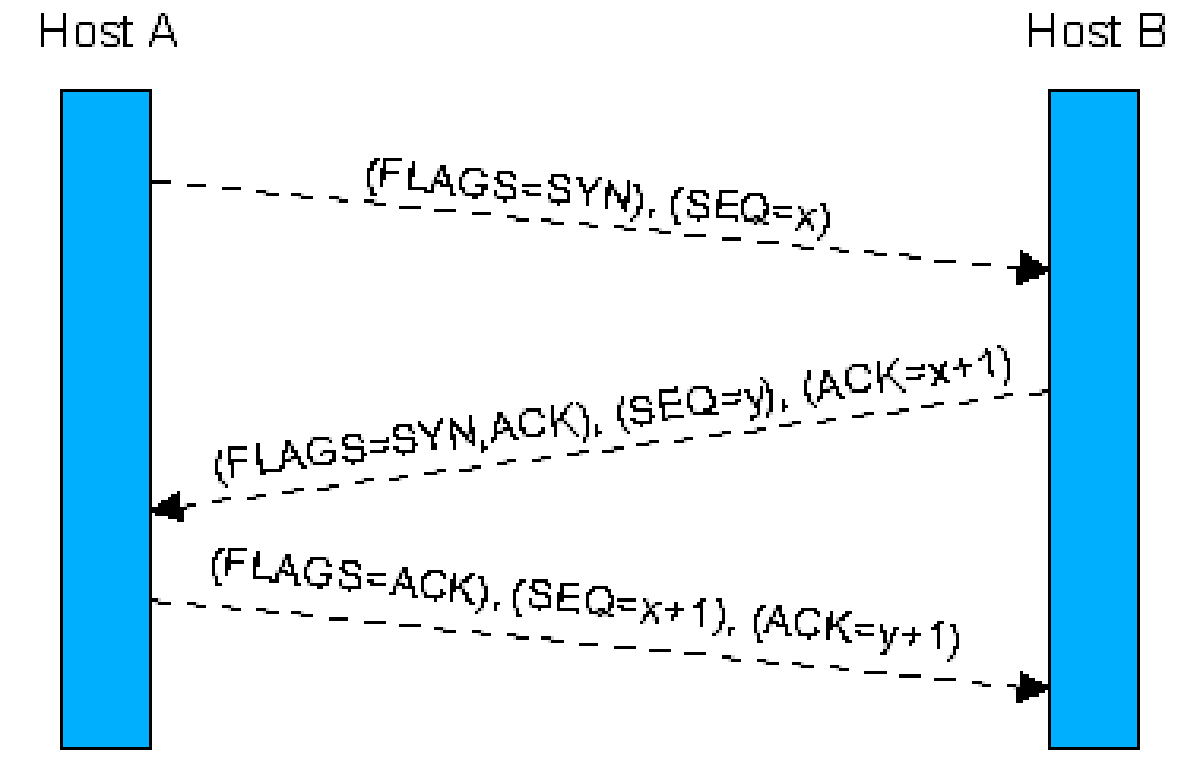
\includegraphics[scale=0.35]{images/ThreeWayHandshake.png} 
\end{center}
    \caption{three-way handshake \cite{noauthor_einfuhrung_nodate}}
    \label{img:three-way handshake}
    
\end{figure}
\subsection{TCP-Client} \label{TCP-Client} %Schreibweise ?
\subsubsection{Übersicht}
Der TCP-Client stellt Clientverbindungen für TCP-Netzwerkdienste bereit. Die TCP-Client Klasse bietet einfache Methoden zum Herstellen einer Verbindung, senden und empfangen von Daten. Der TCP-Client verbindet sich mit einem TCP-Listener und stellt danach einen Network Stream zur Verfügung, welcher ausgelesen werden kann und auf welchem geschrieben werden kann. Zum Verbinden mit einem TCP-Listener gibt es zwei Möglichkeiten:
Der TCP-Client stellt “Connect” Methoden zur Verfügung, oder man kann im Konstruktor bereits die IP-Adresse und den Port angeben. Im Konstruktor wird dann die Verbindung automatisch hergestellt.
Wenn die Verbindung besteht, kann mit .GetStream() der Network Stream des TCP-Clients abrufen und diesen mit .Read(Byte[],Int32,Int32) auslesen oder diesen mit .Write(Byte[],Int32,Int32) beschreiben. Wenn der Kommunikationsaustausch abgeschlossen ist, sollte der TCP-Client mit .Close(Int32) geschlossen werden.
\subsubsection{Konstruktoren}
Name: \textbf{TCPClient()}
\newline
Info: Erstellt einen TCP-Client, der noch zu keinem TCP-Listener verbunden ist.
\newline
\newline
Name: \textbf{TCPClient(IPEndpoint)}
\newline
Info: Erstellt einen TCP-Client, welcher sich im Konstruktor bereits zu dem angegebenen IPEndpoint verbindet.
\newline
\newline
Name: \textbf{TCPClient(string, Int32)}
\newline
Info: Erstellt einen TCP-Client, welcher sich im Konstruktor bereits zu der als String angegebenen IP-Adresse und dem als Int32 angegebenen Port verbindet.
\subsubsection{Methoden}
Name: \textbf{Close()}
\newline
Info: Schließt die Verbindung zum Remotehost.
\newline
\newline
Name: \textbf{Connect()}
\newline
Info: Verbindet den TCP-Client mit dem Remotehost. Dazu gibt es verschiedene Parameter:
\newline \tab \newline
- \textit{Connect(IPAdress, Int32)}, wobei hier die IP-Adresse bereits als IPAdress-Objekt und der Port als Int32 mitgegeben wird.
\newline \tab \newline
- \textit{Connect(IPAdress[], Int32)} wird benutzt wenn der Remotehost mehrere DNS-Einträge hat und man nicht genau weiß, welcher der richtige ist. Es wird eine Liste aller IP-Adressen mitgegeben, wobei es sich auch hier um IPAdress-Objekte handelt. Auch hier wird der Port als zweiter Parameter als Int32 mitgegeben.
\newline \tab \newline
- \textit{Connect(IPEndPoint)}: Hier wird direkt ein IPEndPoint-Objekt mitgegeben, welches bereits alle relevanten Infos über den Remotehost beinhaltet.
\newline \tab \newline
- \textit{Connect(string, Int32)}: Die einfachste Methode, da hier die IP-Adresse einfach als String mitgegeben wird. Auch hier wird als zweiter Parameter der Port als Int32 angegeben.
\newline
\newline
Name: \textbf{ConnectAsync()}
\newline
Info: Verbindet den TCP-Client mit dem Remotehost asynchron. Dazu gibt es verschiedene Parameter:
\newline \tab \newline
- \textit{ConnectAsync(IPAdress, Int32)}, wobei hier die IP-Adresse bereits als IPAdress-Objekt und der Port als Int32 mitgegeben wird.
\newline \tab \newline
- \textit{ConnectAsync(IPAdress[], Int32)} wird benutzt wenn der Remotehost mehrere DNS-Einträge hat und man nicht genau weiß welcher der richtige ist. Es wird eine Liste aller IP-Adressen mitgegeben, wobei es sich auch hier um IPAdress-Objekte handelt. Auch hier wird der Port als zweiter Parameter als Int32 mitgegeben.
\newline \tab \newline
- \textit{ConnectAsync(string, Int32)}: Die einfachste Methode, da hier die IP-Adresse einfach als String mitgegeben wird. Auch hier wird als zweiter Parameter der Port als Int32 angegeben.
\newline \newline
Name: \textbf{Dispose()}
\newline
Info: Gibt alle vom TCP-Client verwendeten Ressourcen frei.
\newline \newline
Name: \textbf{GetStream()}
\newline
Info: Gibt den Network Stream zurück, welcher für das Senden und Empfangen von Daten wichtig ist.
\newline
\subsubsection{Verwendung in Ludimus}
Die Verbindung zwischen Smartphone und Server(PC/Laptop) baut auf einem Network Stream auf, also ist es notwendig die Verbindung per TCP-Client und TCP-Listener durchzuführen. Zusätzlich bietet TCP, hier viele Vorteile weshalb die Wahl zum TCP-Client nicht schwer fiel. In Ludimus ist jedes Smartphone, welches sich mit dem Server, per TCP-Verbindung, verbindet, ein TCP-Client, welcher in einer Liste gespeichert wird und so für jeden zur Verfügung stehen. Zusätzlich gibt es die .SendData(string key,string value) Methode welche den Zugriff auf den Network Stream über den TCP-Client löst.
\subsection{TCP-Listener} \label{TCP-Listener}
\subsubsection{Übersicht}
Die TCP-Listener Klasse bietet einfache Methoden, die das akzeptieren von eingehenden Verbindungsanfragen erlauben. Die TCP-Listener Klasse wird zusammen mit dem TCP-Client benutzt, um eine Verbindung miteinander aufzubauen und per Network Stream zu kommunizieren. Dem TCP-Listener selbst wird dabei im Konstruktor als Parameter die IP-Adresse und der Port, auf welchem der TCP-Listener hören soll, mitgegeben. Als IP-Adresse kann auch Any mitgegeben werden, um den TCP-Listener auf der lokalen IP-Adresse laufen zu lassen. Um den TCP-Listener zu starten, muss einfach .Start() aufgerufen werden und somit horcht der TCP-Listener auf der angegeben IP-Adresse und Port. Eingehende Verbindungsanfragen werden in eine Warteschlange gereiht. Mit .AcceptSocket() oder .AcceptTCP-Client() wird die erste Verbindungsanfrage aus der Warteschlange genommen und kann dann an einen TCP-Client weitergegeben werden. Die .AcceptSocket() und .AcceptTCP-Client() Methoden blockieren jedoch und warten bis auch wirklich eine Verbindungsanfrage kommt. Diese beiden Methoden in einen Thread auslagern macht durchaus Sinn. Wenn man jedoch keinen Thread benutzen will, kann man auch einfach mit der .Pending() Methode abfragen, ob in der Warteschlange eine Verbindungsanfrage eingereiht ist. Mit der .Stop() Methode kann der TCP-Listener gestoppt werden. Die .Stop() Methode jedoch schließt nicht alle vorhandenen TCP-Client Verbindungen. Diese danach noch sauber zu schließen liegt in der Hand des Programmierers.
\subsubsection{Konstruktoren}
Name: \textbf{TCPListener(Int32)}
\newline
Info: Erstellt einen TCP-Listener, welcher auf dem als Int32 angegebenen Port horcht.
\newline \newline
Name: \textbf{TCPListener(IPAdress, Int32)}
\newline
Info:  Erstellt einen TCP-Listener, welcher auf der lokalen, als IPAdress Objekt übergebenen IP-Adresse und dem als Int32 angegebenen Port horcht.
\newline \newline
Name: \textbf{TCPListener(IPEndpoint)}
\newline
Info: Erstellt einen TCP-Listener, welcher auf dem angegebenen IPEndpoint horcht.
\newline \newline
\subsubsection{Methoden}
Name: \textbf{AcceptSocket()}
\newline
Info: Gibt den ersten Socket in der Request-Warteschlange zurück. Blockiert den Thread, in welchem die Methode aufgerufen wurde.
\newline \newline
Name: \textbf{AcceptSocketAsync()}
\newline
Info: Gibt den ersten Socket in der Request-Warteschlange zurück. Wird asynchron ausgeführt.
\newline \newline
Name: \textbf{AcceptTCPClient()}
\newline
Info: Gibt den ersten TCP-Client in der Request-Warteschlange zurück. Blockiert den Thread, in welchem die Methode aufgerufen wurde.
\newline \newline
Name: \textbf{AcceptTCPClientAsnyc()}
\newline
Info: Gibt den ersten TCP-Client in der Request-Warteschlange zurück. Wird asynchron ausgeführt.
\newline \newline
Name: \textbf{Start()}
\newline
Info: Der TCP-Listener startet und wartet ab jetzt auf eingehende Verbindungsanfragen.
\newline \newline
Name: \textbf{Stop()}
\newline
Info: Der TCP-Listener stoppt und horcht nicht mehr auf eingehende Verbindungsanfragen. Wichtig: Durch Stop werden die TCP-Client Verbindungen nicht sauber geschlossen.
\newline \newline
\subsubsection{Implementierung in Ludimus}
Beim Starten der PC/Laptop App wird ein TCP-Listener gestartet, welcher auf die eingehenden Verbindungsanfragen der Smartphones, auf welchen ein TCP-Client läuft, horcht. Der TCP-Listener nimmt maximal acht Verbindungen an. Er wird in einem extra Thread geöffnet, welcher permanent im Hintergrund läuft. Somit wird, bis acht Verbindungen erreicht wurden, permanent auf Verbindungsanfragen geachtet. Wenn eine Verbindungsanfrage ankommt wird sie mit hilfe der .AcceptTCP-Client() Methode angenommen und einem Player-Objekt übergeben.
\subsection{Network Streams} \label{ns}
\subsubsection{Übersicht}
Network Ressourcen werden im .Net Framework als Streams angesehen, diese heißen Network Streams. Eigenschaften von Network Streams sind unter anderem, dass egal welchen Datentyp sie senden oder lesen, dies mit den .Write() und .Read() Methoden möglich ist. Außerdem sind sie sehr ähnlich den anderen im .Net Framework oft benutzten Streams. Der einzige Unterschied ist, dass die Network Streams nicht suchbar sind. Die .Seek() und .Position() Methoden werfen bei Network Streams eine NotSupportedException. Network Streams sind ein Teil des System.Net.Sockets Namespaces. Die Network Stream Klasse bietet Methoden für das Senden und Empfangen von Daten, dabei hat die Network Stream Klasse Methoden für asynchrones und synchrones Senden und Empfangen. Um einen Network Stream zu bekommen muss bereits vorher eine Socket oder TCP Verbindung zwischen den beiden kommunizierenden Geräten vorhanden sein. Zu beachten ist, dass wenn man den Network Stream schließt nicht automatisch auch die Socket oder TCP Verbindung geschlossen wird, sondern der Programmierer diese noch extra sauber schließen muss. Um das ganze synchron zu machen, reichen die oben bereits angesprochenen .Write() und .Read() Methoden, die allerdings den jeweiligen Thread blockieren. Um das ganze asynchron zu machen, sollte man die .BeginRead()/.EndRead() und .BeginWrite()/.EndWrite Methoden benutzen. Diese geben ein IAsyncResult zurück und sind damit dafür besser geeignet. Solange man jedoch einen eigenen Thread für die .Write() und für die .Read() Methode hat können beide synchron auf dem Network Stream eingesetzt werden.
\subsubsection{Methoden}
Name: \textbf{Close(Int32)}
\newline
Info: Schließt den Network Stream nach einer, durch Parameter angegebenen, Zeit in welcher noch Daten über den Network Stream gesendet werden.
\newline \newline
Name: \textbf{CopyTo(Stream,Int32)}
\newline
Info: Kopiert den gesamten Network Stream in einen anderen Stream, welcher durch die Parameter angegeben wird. Zusätzlich kann, in Form eines Int32, auch eine Buffergröße angegeben werden, diese dient zur Beschränkung des kopierten Bereichs.
\newline \newline
Name: \textbf{Dispose()}
\newline
Info: Gibt alle vom Network Stream benutzten Methoden frei.
\newline \newline
Name: \textbf{Flush()}
\newline
Info: Löscht die kompletten Daten des Streams.
\newline \newline
Name: \textbf{Read(Byte[],Int32,Int32)}
\newline
Info: Liest den Network Stream aus. Das Byte Array gibt dabei den Buffer an, in welchem die empfangenen Daten geschrieben werden. Der zweite Parameter an welcher Stelle angefangen wird in den Buffer zu schreiben und der dritte Parameter legt fest wie viel eingelesen werden soll.
\newline \newline
Name: \textbf{Write(Byte[],Int32,Int32)}
\newline
Info: Schreibt in den Network Stream. Das Byte Array gibt dabei den Buffer an, der die Daten gespeichtert hat, die versendet werden sollen. Der zweite Parameter an welcher Stelle des Buffers angefangen wird zu senden und der dritte Parameter legt fest wie viel vom Buffer versendet werden soll.
\newline \newline
\section{Sonstige Technologien}
\subsection{Figma (DM)} \label{sec:figma}
Figma ist ein Online Mockup Tool zum schnellen Erstellen von Userinterfaces. Entwürfe werden über die Cloud synchronisiert und können von mehreren Benutzern kollaborativ verwendet werden. Durch die Verfügbarkeit im Browser und das ermöglichen von Gruppenarbeiten, entschieden wir uns für Figma anstatt für Illustrator, welches wir noch zu Beginn benutzten.
\subsection{Blender}
Blender ist ein Open Source 3D-Modellierungstool. Es ist gratis nutzbar und bietet neben der Modellerstellung noch viele weitere wichtige Features, wie Animationen, Materialerstellung oder die Kolorierung von Objekten. Durch die in Punkt \ref{sec:unity-blender} angesprochene Synergie, zwischen Blender und Unity, ist der Importprozess reibungslos.
\subsection{Vectr (DM)}
Vectr ist ein einfaches Tool zum Erstellen von Vector Grafiken. Die Funktionalität ist zwar auf ein paar Formen und Textfelder beschränkt, jedoch war dies ausreichend für all unsere Icons, weshalb wir von Photoshop zu Vectr wechselten.
\subsection{Illustrator (DM)}
Zu Beginn des Projektes benutzten wir Illustrator noch für die Mockup Erstellung. Wie in Punkt \ref{sec:figma} erwähnt, änderte sich dies jedoch und Illustrator wurde nur für die Erstellung des Billiardtisches, aufgrund der Mustererstellung für das Tuch, die Holzränder und die Metallecken, genutzt.
\subsection{Delegates (ES)}
\subsubsection{Übersicht}
Ein Delegat ist ein Typ, der Verweise auf Methoden mit einer bestimmten Parameterliste und dem Rückgabetyp darstellt. Nach Instanziierung eines Delegaten können Sie die Instanz mit einer beliebigen Methode verknüpfen, die eine kompatible Signatur und einen kompatiblen Rückgabetyp aufweist. Sie können die Methode über die Delegatinstanz aufrufen.
Delegaten werden verwendet, um Methoden als Argumente an anderen Methoden zu übergeben .Ereignishandler sind nichts weiter als Methoden, die durch Delegaten aufgerufen werden.
\subsubsection{Anwendung}
Um ein Delegate nutzen zu könnenen muss zuerst ein delegate erzeugt werden:
\newline
\tab public delegate string DoSth(string name, int y);
\newline
Beim erstellen des Delegates wird nach dem Keyword “delegate” der Rückgabewert der Methode bestimmt, in diesem Fall wird String zurückgegeben. Darauf folgt der Name, in unserem Fall “DoSth”, danach werden die Parameter welche die Methode benötigt noch angegeben und fertig ist das Delegate. Um dieses jedoch auch benutzen zu können muss es noch instanziiert werden. Dies kann man mit: public DoSth doSthHandler;. Nun kann das Delegate erst richtig benutzen. Nun kann dem Delegate eine Methode welche der obigen ovn der Signatur gleich hinzugefügt werden. Dies kann ganz einfach mit DoSth += myMethod; geschrieben werden. Wurde die Methode zum Delegate hinzugefügt kann man sie und alle anderen Methoden auf dem delegate mit: this.DoSth(“Parameter 1”, Parameter 2); aufrufen.
\subsubsection{Implementierung in Ludimus}
Bei Ludimus werden solche Delegates benutzt um Schnittstellen nach außen bereits zustellen. Diese Schnittstellen können benutzt werden um zum Beispiel eine Methode zum Player InputHandler hinzufügen und so aufgrund des gesendeten Key-Value Pair, des Smartphones, kann man selbst Befehle ausführen und zum Beispiel einen Charakter bewegen. Zusätzlich bietet die Nutzung von Delegates den großen Vorteil das man den Input auf jedes Spiel anpassen kann und somit Keywords, wie “move”, welche von mehreren Spielen verwendet werden öfters zu verwenden kann, da die Abfrage auf diese nicht von der Grundplattform durchgeführt wird sondern vom jeweiligen Spielscript.
\subsection{ZXing.Net (ES)}
\subsubsection{Übersicht}
Um einen QR-Code in C Sharp zu erzeugen wurde die ZXing.Net Library benutzt, welche die Entschlüsselung und Erzeugung von Barcodes unterstützt. ZXing.Net ist der Port der Java basierenden Library ZXing welche ebenfalls für Barcodes benutzt wird.
\newline \newline
ZXing.Net unterstütz eine Vielzahl von Barcode-Entschlüsselungen, um genau zu sein Unterstützt es: UPC-A, UPC-E, EAN-8, EAN-13, Code 39, Code 93, Code 128, ITF, Codabar, MSI, RSS-14 (all variants), QR Code, Data Matrix, Aztec and PDF-417.
\newline \newline
Der Barcode-Erzeuger unterstützt: UPC-A, EAN-8, EAN-13, Code 39, Code 128, ITF, Codabar, Plessey, MSI, QR Code, PDF-417, Aztec, Data Matrix
\subsubsection{Einbindung}
Grundsätzlich kann man die Library als NuGet Package downloaden. Dies ist jedoch in Unity nicht möglich. In Unity wird das ganze mithilfe einer .dll File gemacht welche in den Plugins-Folder in Unity gezogen wird. Schon kann man sie in den C Sharp Scripts benutzten.
\subsubsection{Warum ZXing.Net}
Die XZing.Net Library beitet eine Einbindung in Unity an und sie ist in C Sharp geschrieben. Sie ist  somit die einzige QR-Code Library welche es kostenfrei ermöglicht QR-Codes, in C Sharp zu erstellen und zu entschlüsseln. Einziger Negativpunkt ist die teils mangelnde Dokumentation.
\subsubsection{Usage}
\paragraph{Erzeugung}
In Unity muss man zur Benutzung der Library eine WebCamTexture instanzieren. Diese kann man mit “.Play()” und “.Stop()” starten und anhalten. Um nun aus der WebCamTexture Pixel auszulesen wird die Methode “.GetPixels32()” angewandt. Diese lieftert ein Color32 Array zurück. Mit diesem Array selbst fängt man wenig an, da es einfach nur ein Array von Farbwerten ist. Um mit dem Array arbeiten zu können muss zusätzlich noch einen IBarcodeReader instanziert werden. Dies geht mithilfe der “BarcodeReader()” Methode welche ZXing.Net beinhaltet und eben genau einen IBarcodeReader zurück gibt. Zum Entschlüsseln des Barcodes wird einfach die “.Decode(Color32 Array, WebCamTexture Höhe, WebCamTexture Breite)” Methode benutzt welche einen String, welcher den entschlüsselten QR-Code als Text beinhaltet, zurückliefert. Dieser wird das Color32 Array welches vorher erzeugt wurde als erster Parameter mitgegeben. Zusätzlich benötigt die Methode noch die Höhe und Breite der bereits instanzierten WebCamTexture. Dies geht dank den Properties der WebCamTexture “.height” und “.width”  ganz einfach. Um herauszufinden ob ein Barcode gefunden wurde wird einfach das Ergebnis der Decode Methode mit null verglichen, da es leer ist wenn kein Code gefunden wird.
\paragraph{Entschlüsselung}
Bei dem Erzeugen von Barcodes wird zunächst eine leere 2DTexture erzeugen, diese dient als an Anzeigefläche für den QR-Code. Darauf wird nun mit hilfe eines BarcodesWriters, welchem das Format “BarcodeFormat.QR\_CODE” zugewiesen wird und als Optionen die Höhe und Breite der 2DTexture mitgegeben werden. Mithilfe der “.Write(Text)” Methode bekommt man ein Color32 Array zurück, welches nun auf die 2DTexture geschrieben wird.
Nun wird diese noch im Frontend angezeigt und schon hat man einen QR-Code erzeugt.
\subsubsection{Implementierung in Ludimus}
Bei der Implementierung in Unity gab es ein gewaltiges Problem. Die Kamera war während der Anzeige im Frontend, wegen der Berechnung der ZXing.Net Library, ob ein Code gefunden wurde, nicht flüssig. Es wurden immer nur im Sekundenabstand Frames angezeigt. Auch wenn das reicht um den QR-Code zu scannen war es bei weitem nicht genug um auch benutzbar zu sein. Die Lösung war einfach einen Kamerastream zu zeigen mit welchem nichts berechnet wurde und welcher somit flüssig war.Dies jedoch klingt leichter als gedacht, denn in man kann in jeder Unity-Scene nur eine WebCamTexture am laufen haben. Als Endlösung wird in der Unity-Scene bereits eine WebCamTexture gestartet und dann die Berechnung des QR-Codes, mit einer neuen WebCam


\chapter{How to use (ES)}
\section{Vor dem Start}
Da die Ludimus-App ihre Verbindungen innerhalb des lokalen Netzwerks aufbaut, ist Voraussetzung, dass sich alle Geräte, auf denen der User Ludimus benutzten möchte, in einem lokalen Netzwerk befinden. Dies kann erreicht werden, indem man die Endgeräte alle mit dem gleichen W-Lan Netzwerk verbindet oder man sich einen Hotspot auf dem Smartphone erstellt und die Geräte damit verbindet. Zusätzlich muss auf allen Geräten, welche zum Spielen benutzt werden möchten, die Ludimus-App installiert sein. Dazu zählt auch der Laptop/Pc/SmartTv den man als Bildschirm benutzen möchte.
\section{Computer-App}
Wenn alle generellen Bedingungen erfüllt sind, kann man die Ludimus-App auf dem PC/Laptop starten. Nach einer kurzen Ladezeit wird dort den Usern ein Lobbycode und ein QR-Code angezeigt. Diese werden für die Verbindung mit dem Smartphone wichtig und da das Smartphone als Fernbedienung für die App fungiert kann der User sich nun zurücklehnen und bequem Ludimus bedienen.
\section{Android/IOS - App}
\subsection{Vor dem Einloggen}
Beim Starten der Ludimus-App öffnet sich zunächst die Login Maske, in welcher man gebeten wird sich einzuloggen. Wenn der User sich bereits einen Account erstellt hat, muss er nur seine Daten in der Maske ausfüllen und auf den Login Button drücken, um sofort erfolgreich eingeloggt zu werden. Wurde noch kein Account erstellt, hat der User zwei Möglichkeiten: Er kann sich einen neuen Account erstellen oder sich als Guest anmelden. Entscheidet er sich für die Variante Guest, hat er selber keine Spiele selbst zur Verfügung sondern kann nur Spielern mit bezahltem Account beitreten. In den Spielen ansich gibt es keinen Unterschied zwischen Guest und zahlendem Benutzer. Um sich einen Account zu erstellen, muss der auf den Sign-Up Button drücken. Es öffnet sich eine neue Maske, in welcher E-Mail und Passwort einzugeben sind. Aus Sicherheitsgründen wird die Eingabe des Passworts zweimal verlangt. Zum Erstellen des Accounts muss er die Eingabe mit Klick auf den nun rechts platzierten Sign-Up Button bestätigen. Der Account wird automatisch in der Firebase-Datenbank gespeichert und man wird sofort eingeloggt.
\subsection{Nach dem Einloggen}
Wenn der Spieler eingeloggt ist, kann er einen Namen und einen Lobbycode eingeben, dieser wird in der gestarteten Ludimus-App für den PC/Laptop angezeigt. Alternativ kann man auch den QR-Code, der den Lobbycode hinterlegt hat und ebenfalls in der Ludimus-App für PC/Laptop angezeigt wird, scannen und sich noch einfacher mit dem Server verbinden. Zum Scannen des QR-Codes klickt man auf den entsprechenden Button, es öffnet sich eine Kamera in der App und der QR-Code wird eingelesen. Sind beide Felder ausgefüllt hat, kann man sich mit einem Klick auf das W-Lan Symbol zu dem Server verbinden. Bei erfolgreicher Verbindung gibt es zwei Varianten. Möglichkeit 1: Der erste Spieler der sich zum Server verbindet ist der Admin der Lobby und kann Spiele starten und downloaden. Spiele werden per Klick auf das Symbol im Hauptmenü gestartet und damit auf allen Smartphones und auf dem PC/Laptop geladen. Möglichkeit 2: 
Man ist nicht der Admin der Lobby, sondern lediglich Mitspieler. In dieser Rolle wartet man, bis der Admin das Spiel startet, und dieses automatisch auf dem Smartphone lädt.

\chapter{Ausgewählte Aspekte der Systemerstellung}
\section{Designentscheidungen (DM)}
Ludimus war von Beginn an als ein Produkt für Konsumenten gedacht, weshalb wir viele Überlegungen und anschließende Änderungen bezüglich der Benutzeroberfläche anstellten. Viele der Abwandlungen sind mit dem Hintergedanken der Benutzbarkeit der Plattform verbunden und konzentrierten sich auf Farben, sowie Form und Anordnung. Im Folgenden Abschnitt werden generelle Designentscheidungen beschrieben, die sich auf alle Aspekte es Projekts ausgewirkt haben. Änderungen die nur einen Teilbereich umfassten, werden in Punkt \ref{sec:special-design} genauer erwähnt.
\subsection{Generelle Designentscheidungen}
\begin{center}
    \begin{figure}
        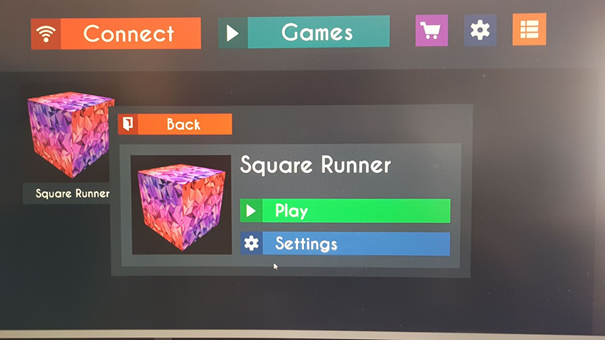
\includegraphics[scale=0.7]{images/design01.png} 
        \caption{Erster Shop Prototyp}
        \label{img:design01}
    \end{figure}
\end{center}
Für die ersten Iterationen des Projekts wählten wir dunkle Farben um auch das Spielen in den späteren Stunden zu ermöglichen. Die Grafik \ref{img:design01} zeigt das Server Interface, wobei hier das Shop-Interface zu sehen ist, sowie die Detailansicht eines Spieles. 
\newline
\begin{center}
    \begin{figure}
        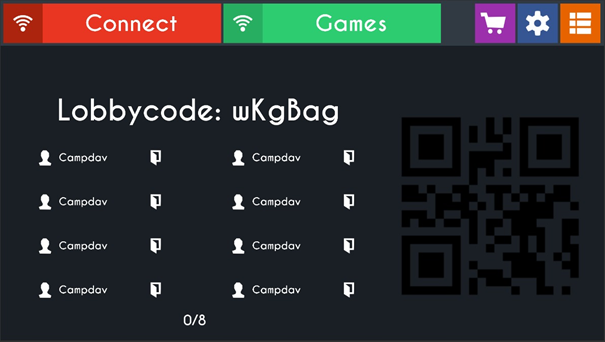
\includegraphics[scale=0.7]{images/design02.png} 
        \caption{Lobby Prototyp}
        \label{img:design02}
    \end{figure}
\end{center}
Um einerseits mehr Platz für den eigentlichen Inhalt zu haben und andererseits moderner auszusehen, änderten wir die Proportionen, die Abstände und Teils die Farben, um an die Kacheln von Windows 8, zu erinnern, wie in der Abbildung \ref{img:design02} zu sehen. Hier ist die Lobbyansicht ausgewählt. 
\newline
\begin{center}
    \begin{figure}
        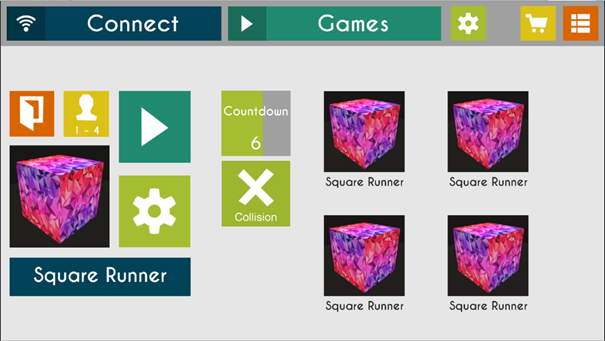
\includegraphics[scale=0.7]{images/design03.png} 
        \caption{Shopdetailansicht mit Einstellungen und hellem Farbschema}
        \label{img:design03}
    \end{figure}
\end{center}
Ludimus war Primär als Produkt für Familien mit Kindern gedacht. Dunkle Farben übermittelten nicht das Gefühl, das wir transportieren wollten, weshalb wir uns für helle Farben auf weißen Hintergrund entschieden. \ref{img:design03} zeigt auch eine Umgestaltung der Detailansicht, dazu jedoch in Punkt \ref{sec:shop} mehr.
\newline
\begin{center}
    \begin{figure}
        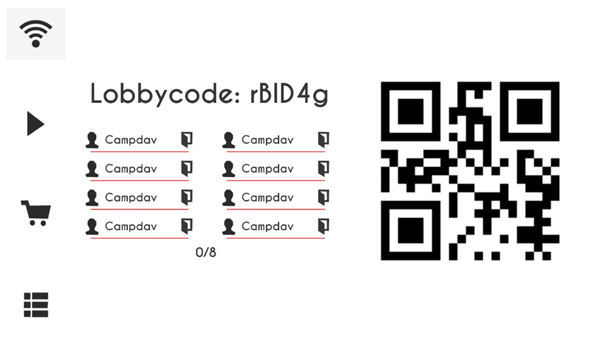
\includegraphics[scale=0.7]{images/design04.png} 
        \caption{Schwarz-Weiß Designentwurf}
        \label{img:design04}
    \end{figure}
\end{center}
Einen gewissen Rückschritt in Sachen Farben stellte unser nächstes UI dar, zu sehen in \ref{img:design04}. Der Hintergedanke hierbei war die Vereinfachung der Plattform und ein schwarz-weißes Design half uns dabei. Nutzer sahen nun auch erstmals, in welchem Menü sie sich befanden, da dieses nun einen dunkleren Hintergrund bekam. Globale Einstellungen für die Plattform selbst als eigener Punkt, wurden mit diesem Design entfernt.
\newline
\begin{center}
    \begin{figure}
        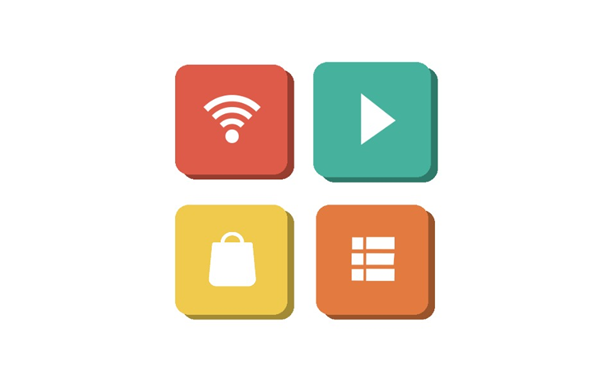
\includegraphics[scale=0.7]{images/design05.png}
        \caption{Buntes Hauptmenü mit Schatten und abgerundeten Ecken}
        \label{img:design05}
    \end{figure}
\end{center}
In den nächsten Iterationen brachten wir einerseits Farbe zurück, rundeten andererseits aber auch alle Buttons ab und gaben ihnen einen Schatten, wie in \ref{img:design05} zu sehen. Hatte man in allen bisherigen Versionen noch eine Menüleiste und einen Inhaltsteil, so entfernten wir Erstere um nur den Inhalt darstellen zu können. Drückt der Nutzer nun auf einen der vier Menüpunkte, so schwenkt die Kamera in dessen Ecke und der Inhalt wird dort angezeigt. Mit einem Zurück-Knopf kann der Benutzer anschließend wieder zum Hauptmenü gelangen. Wir implementierten zusätzlich noch eine Farbauswahl für das gesamte Interface. Benutzer konnten sich bestimmte Farbkombinationen auswählen, um sowohl die vier Primärfarben, als auch den Hintergrund zu ändern. Diese Entscheidungen hatten jedoch alle mehrere Nachteile, weshalb wir alles wieder verändern mussten. Die Kameraanimationen waren zwar interessant anzusehen, jedoch verlangsamten sie den Navigationsprozess Unnötigerweise. Zusätzliche Probleme machten verschiedene Formate, da die Animationen nur auf 16:9 optimiert waren. Obwohl das Farbschema wechseln gut funktioniert hat und Menschen mit verschiedenen Präferenzen die Möglichkeit gab das UI zu verändern, mussten wir das Feature entfernen, da uns die Erkennung unserer Marke wichtig war und wir erreichen wollten, dass sobald Familien unser Logo oder unsere Farben sehen an uns denken können. Wenn jeder seine eigenen Farben festlegen kann, ist dies nicht möglich.
\newline
Bisher waren eine Übersicht der Lobby, der Shop, alle Heruntergeladenen Spiele und ein Menü für Optionen in der Serveransicht und der Client konnte nur Name und Lobbycode eingeben und sich anschließend verbinden. Wollte eine Gruppe also spielen, mussten sich zuerst alle Spieler auf deren Handys zum großen Bildschirm verbinden und danach musste ein Spieler das Tablet, den Laptop oder den Fernseher bedienen um ein Spiel zu starten, oder zuerst herunterladen. Speziell beim Spielen im Wohnzimmer über den Fernseher gibt es hier enorme Probleme, die mit der Steuerung von Menüs mit der Fernbedienung zu tun haben. Um diese unnötige Interaktion mit dem großen Bildschirm zu entfernen, gestalteten wir die Aufteilung der Menüs komplett um. Der Server sollte nur noch die Lobby anzeigen, da diese keine Interaktion forderte. Sowohl Spielernamen, als auch der Lobbycode in schriftlicher und grafischer Form, konnten so größer dargestellt werden. Zusätzlich zu einem Login Fenster, welches wir bei App-Start dem Client hinzugefügt haben, wurden Spieler wie immer aufgefordert ihren Namen und den Lobbycode einzugeben um sich anschließend zu verbinden. Dieser Vorgang blieb für alle Spieler bis auf den ersten gleich. Dieser hat nun jedoch die Kontrolle über die Lobby und kann sowohl neue Spiele herunterladen, als auch bereits heruntergeladene Spiele starten. Um das Interface zu vereinfachen, vereinten wir den Shop mit den heruntergeladenen Spielen. Durch den Verzicht einer einheitlichen Trennung kann der Nutzer nicht unterscheiden ob ein Spiel zuerst heruntergeladen werden muss und probiert so viel mehr neue Spiele. Die Downloadzeit überschreitet nur selten 10 Sekunden, wodurch dies nur noch verstärkt wird. 
\newline
\begin{center}
    \begin{figure}
        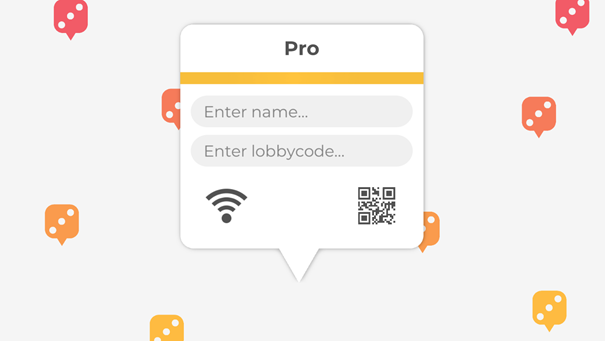
\includegraphics[scale=0.7]{images/design06.png} 
        \caption{UI zum Verbinden zu einer Lobby}
        \label{img:design06}
    \end{figure}
\end{center}
Wie in \ref{img:design06} zu sehen, ist unser Userinterface mit dem Ludimus Logo eng verknüpft, um es so in die Köpfe der Nutzer zu bekommen. Das UI zum Verbinden zu einer Lobby ist in eine Form, die dem Ludimus Logo ähnelt, eingebettet. Zusätzlich steigen im Hintergrund Ludimus Ballone auf, die ihre Farbe in Abhängigkeit des Subskription Levels, des eingeloggten Nutzers, ändern. 

\subsection{Spezielle Designentscheidungen} \label{sec:special-design}
\subsubsection{Shop} \label{sec:shop}
Der Shop änderte sich über die verschiedenen Versionen am meisten, da die richtige Präsentation der Spiele essentiell für den Kauf eines teureren Subskription Plans ist. Die Änderungen gliedern sich in die Anzeige aller Spiele und die Anzeige eines Spieles.
\newline
Zu Beginn wurden alle Spiele in einem Gitter mit Zeilen und Spalten angezeigt, wie in \ref{img:design01} zu sehen. Überlegungen bezüglich Sortierung oder Suche wurden zu diesem Zeitpunkt noch nicht angestellt. Um Nutzern zu ermöglichen nur Spiele einer bestimmten Art zu sehen, erweiterten wir deren Datenmodell um das Feld „Genre“. Zusätzlich vergaben wir einen Farbcode für jedes Genre, um dem Nutzer schnell ersichtlich zu machen um welche Art von Spiel es sich handelt. Da wir die Plattform für externe Entwickler öffnen wollten, um mehr Spiele anbieten zu können, fügten wir die Reiter „New“, „Top“ und „New Update“ hinzu. Der Gedanke hierbei war neue Spiele eine kurze Zeit unter  „New“ anzuzeigen und Spiele, die oft gespielt werden sollten anschließend unter „Top“ zu finden sein. Um auch ältere Spiele wieder beliebt zu machen oder Entwicklern eine zweite Chance geben zu können, falls der ursprüngliche Release nicht funktioniert hat, würden Spiele die neue Updates erhalten unter „New Update“ gezeigt werden. Den Plan externe Entwickler mit einzubeziehen verworfen wir jedoch, wodurch eine solche Gliederung nicht mehr nötig war, da zu wenig Spiele dafür verfügbar wären. Wie in Abbildung \ref{img:design07} zu sehen, vereinfachten wir zusätzlich die Anzeige der Spiele, in dem wir das Icon des Spieles größer machten, die Detailansicht hinter einem Menü versteckten und wir das Genre des Spieles durch die Farbe der Umrandung klar darstellten. Die zwei Eingabefelder, am unteren Ende des Bildschirms, mit dem Knopf in der Mitte gehören zum Debug Modus, der nur für Entwickler ist, dazu mehr in \ref{sec:debug-modus}.
\begin{center}
    \begin{figure}
        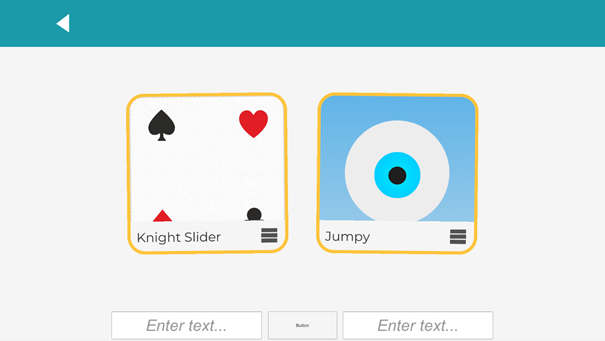
\includegraphics[scale=0.7]{images/design07.png} 
        \caption{Finale Shoppräsentation mit Debug Modus}
        \label{img:design07}
    \end{figure}
\end{center}
Die in Abbildung \ref{img:design03} zu sehenden spielspezifischen Einstellungen wurden entfernt und durch Optionenmenüs im Spiel selbst ersetzt. Durch Änderungen im Startprozess von Spielen wurden Spiele mit mehreren Szenen ermöglicht, wodurch die alte Methode überflüssig wurde.
\section{Spielstart} \label{sec:spielstart}
Sobald der erste verbundene Spieler ein Spiel ausgesucht hat, indem er darauf geklickt hat, und die Gruppengröße für das Spiel in Ordnung ist, wird die ID des Spieles an den Server geschickt.
Dieser sucht sich sowohl die Downloadlinks für die Client-Dateien, als auch für seine eigenen Server-Dateien. Anschließend überprüft er, ob das Spiel schon alle nötigen Dateien für die aktuelle Version heruntergeladen hat. Falls nicht wird das nachgeholt und anschließend werden die Download URLs für die Clients an alle verbundenen Spieler geschickt. Diese überprüfen auch deren Existenz und laden fehlende herunter. Verfügt ein Client über alle Dateien, so schickt er ein „ok“ an den Server. Sobald der Server Bestätigungen aller Clients erhalten hat, startet er seine Szene. Und schickt ein „ok“ an alle Clients, worauf hin diese auch deren Szenen starten. Dieser Ablauf ähnelt dem zwei Phasen Commit bei verteilten Datenbanken, wodurch die Sicherheit dieses Systems bewiesen ist.
\begin{figure}
    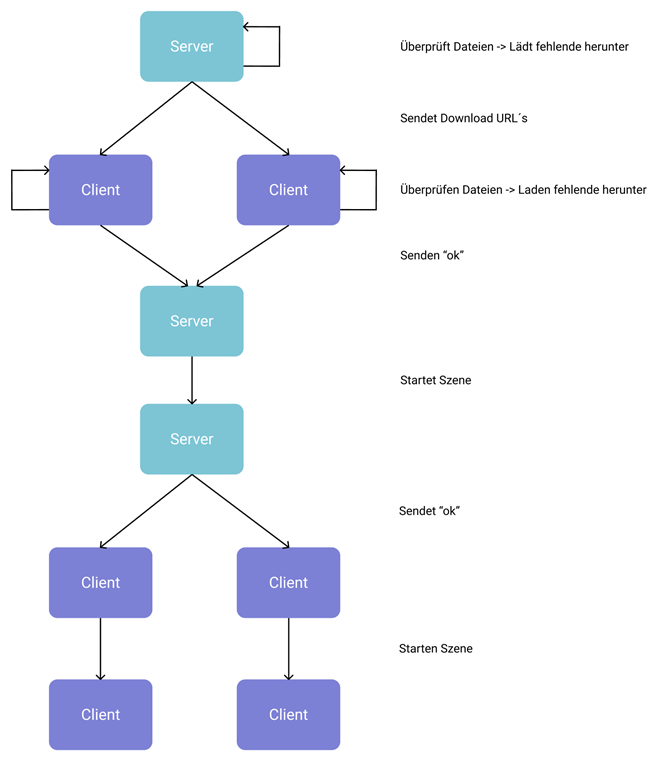
\includegraphics{images/spielstart.png}
    \caption{Vorgang bei Spielstart}
    \label{img:spielstart}
\end{figure}
\subsection{Probleme}
Spiele bestehen drei Komponenten, die gemeinsam dafür sorgen, dass die Spiele funktionieren. Sie bestehen aus Szenen, Modellen und Scripts. Szenen und Modelle, auch Texturen, Materialien, usw. sind in sogenannten „Assetbundles“ gespeichert. Alle Szenen des Clients sind in so einem „Assetbundle“ zusammengespeichert, ähnlich einer Zip-File. Alle Szenen des Server sind ebenfalls so persistiert. Die Unterscheidung zwischen Client und Server ist zwar nicht zwingend nötig, jedoch ist es Ressourcenverschwendung, wenn der Server auch Szenen der Clients speichert, da er diese ohnehin nicht startet, und umgekehrt. Die selbe Speicherung gilt für alle Modelle. Der Grund für die Trennung zwischen Client und Server bleibt gleich, jedoch wäre es deutlich einfacher, wenn Clientszenen und Clientmodelle zusammen gespeichert werden und alle Serverszenen und Servermodelle ebenfalls. Leider unterstützen „Assetbundles“ in Unity diese Funktionalität nicht. 
Als dritter Baustein gelten die Scripts, in denen die Logik der Spiele, das eigentliche Programm, beschrieben ist. Scripts können nicht zu „Assetbundles“ gemacht werden, jedoch gibt es unter Android und Windows die Möglichkeit, sie zu bündeln und dann zur Laufzeit eines Spieles zu verwenden. Unter Ios ist eine derartige Methode nicht möglich, da kein externer Code zur Laufzeit von Apps hinzugefügt werden kann oder darf. Diesen Sicherheitsmechanismus wird Apple nicht entfernen, was bedeutet, dass jeder Code immer in der App vorhanden sein muss. Für den Workflow des Erstellens eines neuen Spieles würde das bedeuten, dass wir alle verwendeten Scripts in das Hauptprojekt transferieren müssen und dann eine neue App Version in den App Store hochladen müssen. Apple User sind ein großer Anteil an unserer Zielgruppe, weswegen ein Ausschluss der Plattform nicht möglich ist. Zwei Speichervarianten für zwei Plattformen, wäre undenkbarer Mehraufwand, weshalb wir uns entschlossen, dass wir für jedes neue Spiel ein Update mit dessen Scripts für alle Plattformen herausbringen.
\subsection{Optimierungsansätze}
Der Fileserver von Firebase hat mit unserem Gratisbezahlplan eine maximale Downloadgröße und eine Grenze für Downloads pro Tag unabhängig von der Größe der Dateien, die heruntergeladen werden. Das ist der Grund, warum nur so viele Zugriffe gemacht werden sollten, wie nötig. Eine Maßnahme war es, dass der Server alle Download URLs beschafft und an die Clients weitergibt. Dieses Prinzip wurde auch für den eigentlichen Download selbst getestet. Im konkreten bedeutet das, dass der Server alle Plattformen der Clients überprüft und dann die Clientdateien für eben diese Plattformen herunterlädt, zwischenspeichert und anschließend den Clients über das lokale Netzwerk sendet. Dieser Ansatz entlastet den Fileserver, da dieser nur einen Downloadrequest verarbeiten muss, der Rest passiert nur zwischen den Spielern. Die gesamte Downloadzeit steigt jedoch dadurch, dass Dateien zwei Mal pro Spieler heruntergeladen werden, anstatt einmal und Clients können während dieser Zeit nur eingeschränkt kommunizieren, weshalb wir uns für die oben beschriebene Variante entschieden.
\section{Debug Modus} \label{sec:debug-modus}
Das in \ref{sec:spielstart} beschriebene System funktioniert einwandfrei mit fertigen Spielen. Da jedoch Spiele sowohl Datenbankeinträge, als auch hochgeladene Dateien am Fileserver benötigen, ist diese Lösung komplett ungeeignet für Spiele in Entwicklung. Der Debug Modus löst dieses Problem und ermöglicht es, auch kleine Änderungen, mit erheblich geringerem Zeitaufwand, zu testen.
Vor dem Debug Modus, wurden die Scripts der fertigen Spiele in das Hauptprojekt hinein kopiert. Die Entwicklung passierte in einem externen Projekt. Diese externen Projekte hatten ein Gerüst, das sich um die Spielerhandhabung und um die Kommunikation zwischen Client und Server im generellen kümmerte. Ein Testdurchlauf der aus „Assetbundles“ für Szenen und Modelle, jeweils wieder unterschieden in Client und Server, bauen, auf Fileserver hochladen, Scripts in Hauptprojekt kopieren und neuste Version für Smartphone und PC bauen dauerte mehrere Minuten.
Mit dem Debug Modus fällt das externe Projekt mit Kommunikationsgerüst, das Bauen der „Assetbundles“ und das hochladen auf den Fileserver weg. Für neue Spiele wird nur ein Ordner im Hauptprojekt und eine Client und Server Startszene angelegt. Die Kommunikation zwischen Server und Client ist mit Delegates abrufbar, wodurch man aktuelle Spieler, deren Inputs und vieles mehr gleich verwenden kann. Bestimmte Aspekte, wie Physics, UI oder Gegner-AI sind Client unabhängig und können somit nun, auch ohne diese, in der Engine, mit einem Knopfdruck, getestet werden. Werden sowohl Client, als auch Server benötigt, die Clients für Smartphone und PC bauen. Der letzte Schritt ist nur bei fast fertigen Versionen nötig, da es sonst eher ratsam ist, nur einen Client zu bauen und den Server in Engine zu debuggen.
Als erster verbundener Spieler kann man in der Spielanzeige das neue Spiel zwar nicht sehen, über die zwei Eingabefelder, kann man jedoch sein Spiel nun starten. Im linken Feld wird der Name der Startszene des Client angegeben und im rechten die des Servers. Drückt der Entwickler nun auf den Knopf in der Mitte wird sein Spiel gestartet. Die Zeiteinsparen und die Erleichterung der Entwicklung sind enorm, weshalb alle fertigen Spiele mit dieser Methode entwickelt worden sind.

\section{Aufbau von Ludimus (ES)}
\subsection{Übersicht}
Ludimus selbst ist in zwei Applikationen unterteilt. Eine läuft auf einem Device, welches man als Controller benutzen will.
Dies kann ein Smartphone (Android/IOS) oder jedes andere Gerät sein, auf welchem Android läuft und wird folglich als Contoller bezeichnet. Die zweite Applikation startet man auf einem Laptop, PC, Tablet oder SmartTV, wodurch das Gerät zum Server wird und weiterführend so bezeichnet wird. Der User muss auf seinem Controller einen Code eingeben oder scannen, um sich zu der Anwendung, welche auf dem Server läuft, verbindet. Der User bedient nach dem Aufbau der Verbindung die komplette Plattform mit seinem Controller. Die Verbindung ist in der Abbildung \ref{img:Ablauf} nochmal detailliert dargestellt.
\begin{figure}
    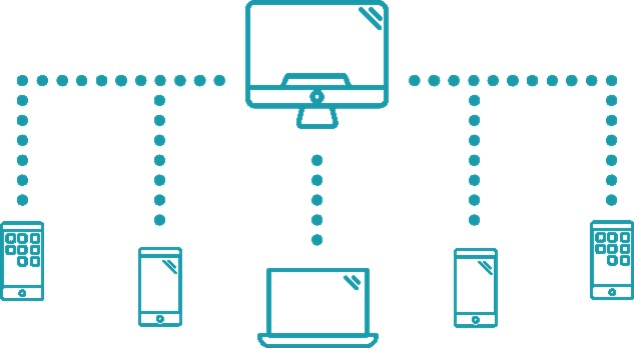
\includegraphics[scale=0.6]{images/ludi.jpg}
    \caption{Aufbau Ludimus}
    \label{img:Aufbau}
\end{figure}
\pagebreak
\subsection{Ablaufdiagram Ludimus}
\begin{figure}
    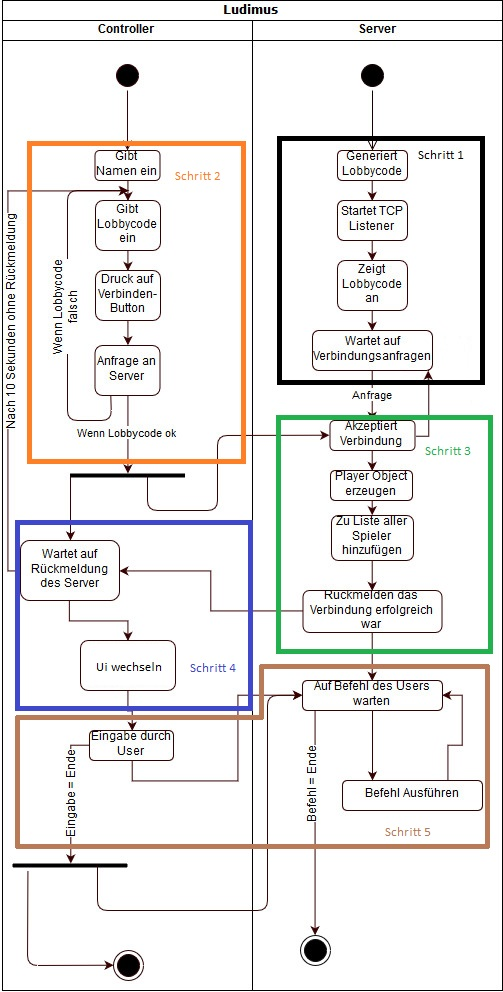
\includegraphics[scale=1.5]{images/Sequence1.jpg}
    \caption{Ablaufdiagram Ludimus}
    \label{img:Ablauf}
\end{figure}
\subsubsection{Erklärung des Ablaufdiagrams(\ref{img:Ablauf})}
\paragraph{Schritt 1}
Im ersten Schritt generiert der Server zunächst einen Lobbycode aufgrund der IP-Adresse des Gerätes.
Genauer ist dies im Kapitel Lobbycodes \ref{lobbycodes} beschrieben. Danach öffnet der Server den TCP-Listener, dies sieht im Code so aus:
\newline \textit{ this.listener = new TCPListener(IPAddress.Parse(this.ipAdress), 9393);\newline
this.listener.Start();}\newline
Wichtig ist hierbei, dass der TCP-Listener nach seiner Instanziierung extra gestartet werden muss. Mehr dazu im Kapitel \ref{TCP-Listener}. Wenn der TCP-Listener erfolgreich gestartet wurde, kann der Lobbycode angezeigt werden, da sich ab diesem Moment Spieler verbinden können. Im Code wird das so realisiert: \newline
\textit{this.LobbyCodeText.text = "Lobbycode: " + this.playermanager.GetLobbyCode();}\newline
Wobei dies in der Initialisierung des UI's und somit in einer anderen Klasse geschieht. Deshalb wird hier auch die
\textit{GetLobbyCode()} Methode des Playermanagers verwendet. \textit{this.LobbyCodeText} ist das TextElement, welches in Unity erzeugt wurde.
Der letzter Teil dieses Schrittes besteht darin, den TCP-Listener „horchen“ zu lassen, damit er auch auf die Anfragen reagieren kann. Code: \newline
\textit{ var tmpClient = this.listener.AcceptTCPClient();} \newline
Dabei ist jedoch zu beachten, dass this.listener.AcceptTCPClient den Mainthread blockiert und solange wartet, bis eine Verbindungsanfrage kommt. Deshalb wird in Ludimus dies in einem eigenem Thread ausgeführt.
\paragraph{Schritt 2}
Bei Schritt 2 gibt der User zunächst seinen Namen und den Lobbycode in die Textfelder des UI's ein. Diese sind per 2-Way Binding mit dem Backend verbunden.
Wenn der User nun auf den Verbindungs-Button drückt, wird der Befehl zum Verbinden ausgeführt, dies sieht im Code wie folgt aus: \newline
\textit{this.client = new TCPClient(DecryptLobbyCode(this.lobbycode), 9393);} \newline
Die \textit{DecryptLobbyCode} Methode wird im Kapitel \ref{lobbycodes} genauer erläutert, der TCP-Client wurde bereits in Kapitel \ref{TCP-Client} behandelt. 9393 definiert den Port, welcher bei Ludimus standardisiert 9393 ist.
\paragraph{Schritt 3}
Der in Schritt 1 bereits beschriebene TCP-Listener akzeptiert mit \textit{this.listener.AcceptTCPClient();} automatisch eine Verbindung, wenn eine Anfrage kommt.
Wird die Verbindung akzeptiert, wird zunächst ein Player Objekt erzeugt. Im Code: 
\newline 
\textit{var tmpPlayer = new Player(); \newline
tmpPlayer.startPlayer(tmpClient, this, this.internalCounter);}
\newline
Hier wird mit new Player() ein neues Objekt erzeugt, welchem dann mittels der \textit{startPlayer()} Methode alle wichtigen Informationen mitgegeben werden, wie der TCP-Client, PlayerManager und Playernumber. In der \textit{startPlayer} Methode wird zusätzlich der Output-Thread geöffnet.
Danach wird das Player Objekt in eine Liste aller Spieler eingefügt, um ständig mit ihm und allen anderen Player Objekten kommunizieren zu können. Am Schluss dieses Schrittes wird dem TCP-Client eine Bestätigung geschickt, dass die Verbindung auch wirklich funktioniert hat. Senden von String im Code:
\newline
\textit{
public void SendData(string key, string value)\{\newline
var dat = new byte[4096];\newline
dat = Encoding.ASCII.GetBytes(key + "|" + value + ";");\newline
this.client.GetStream().Write(dat, 0, dat.Length);\newline
this.client.GetStream().Flush();\newline \}
} \newline
Hier wird zunächst ein Byte-Array der Größe 4096 angelegt. In dieses Byte-Array wird der String, welchen wir senden wollen, geschrieben. 
Dies geschiet mit der \textit{Encoding.ASCII.GetBytes()} Methode in welcher als Parameter der zusendende String steht. 
Der String wird der Methode \textit{SendData} als Key und Value mitgegeben. Mit \textit{this.client.GetStream().Write()} kann man nun auf den Networkstream schreiben.
Wobei man dieser Methode die zu schreibenden Bytes übergibt und angibt, wo angefangen wird zu lesen (da wir vom Anfang lesen wollen 0) und die Länge des zu lesenden Array's übergeben muss.
\paragraph{Schritt 4}
Wenn der TCP-Client, also der Controller, nun die Bestätigung bekommt, wechselt er das UI. In dem neuen UI sieht der Spieler den Ludimus-Shop und alle Spiele, die ihm zur Verfügung stehen.
Empfangen von Daten im Code: \newline
\textit{ 
var data = new byte[4096];\newline
string responseData = string.Empty;\newline
int bytes = stream.Read(data, 0, data.Length); \newline
responseData = Encoding.ASCII.GetString(data, 0, bytes); \newline}
Wichtig ist, dass dies dauerhaft in einem eigenen Thread geschiet, um den MainThread nicht zu blockieren.
Zunächst wird ein neues Byte-Array angelegt, welches 4096 Bytes groß ist. In dieses werden anschließend die gesendeten Daten eingelesen.
Dann muss ein leerer String erzeugt werden, was mit \textit{string.Empty} am saubersten gelöst wird. 
Nun liest man mithilfe von \textit{stream.Read()} in das \textit{data} Array ein. 
Mitgegeben werden dabei das Array, in welches gelesen wird, ein Int, wobei dieser definiert wo im Array angefangen wird einzulesen (in unserem Fall wie bereits erwähnt 0) und die Länge des Arrays in welches gelesen wird.
Mit \textit{Encoding.ASCII.GetString()} wird das Byte-Array zu einem String geparst. 
Dieser String wird in eine Queue gereiht und im MainThread behandelt (siehe \ref{verbindung}). 
Das Lesen von Daten des Network Streams (siehe \ref{ns}) geschieht im Server und Controller auf die gleich Weise.
\paragraph{Schritt 5}
Der letzte Schritt besteht aus dem Warten auf Befehlen am Controller und dem Ausführen von Befehlen am Server.
Es wird zum Beispiel darauf gewartet, dass der User am Controller ein Spiel startet.
Passiert dies, wird mithilfe der in Schritt 3 und 4 beschriebenen Datenübertragung dem Server mitgeteilt, dass er ein Spiel starten soll und dies dann ausführt.
Mehr zu Spielstart unter Kapitel \ref{sec:spielstart}.
\section{Lobbycodes (ES)} \label{lobbycodes}
Das Verbinden zur der Laptop/PC Version von Ludimus erfolgt mit sogenannten Lobbycodes. Dieser wird vom Computer aufgrund der IP-Adresse erzeugt und ermöglicht es einem Smartphone Verbindung zum Rechner aufzubauen.
\subsection{Verbindungsgeschichte}
Die Grundart der Verbindung stand von Anfang an fest, Network Streams, aber wie genau soll sich der User nun, möglichst einfach, mit dem Gerät verbinden? Eine Möglichkeit dafür wäre ein Broadcast, bei solchem wird ein Datenpaket an alle, mit dem gleichen Netzwerk verbundenen Geräte geschickt. Bei Ludimus konkret sollte jedes Gerät gefragt werden ob es die Ludimus-App gestartet hat und sich dann bei erfolgreicher Rückmeldung zu der IP-Adresse des Antwortgeräts verbindet. Dieser Approach ist vermutlich der userfreundlichste, da der User hier nichts selbst machen muss und man sich beim Start der App automatisch zum PC/Laptop verbindet. Jedoch gibt es auch hier mehr als genug Probleme, da es nicht bei jedem Netzwerk mit nur einer Implementierung funktioniert, da einige Netzwerke anders eingestellt sind als andere und somit manchen nicht die Art der C\# Implementierung zulassen. Zusätzlich fehlte uns hier das Wissen um alle Arten eines C\# Broadcasts zu implementieren. Keine Broadcasts aber trotzdem das ganze Netzwerk erreichen? Mit unseren Kenntnissen ein Ding der Unmöglichkeit also muss der User die IP-Adresse irgendwie selbst eingeben, aber wie macht man dies so Userfreundlich wie nur möglich? Nun zum einem durch Kürzung der IP-Adresse und zum anderen durch einen QR-Code, welcher aufgrund der IP erzeugt wird. So kann der User entweder einen kurzen Code eingeben oder gemütlich seine Kamera benutzten zum Scannen des IP-QR-Codes.
\subsection{Erzeugung des Lobbycodes}
Einfach die IP-Adresse eingeben ist dauert aber zu lange da IP-Adressenen nach dem Muster XXX.XXX.XXX.XXX aufgebaut sind und der User somit ganze 12 Zahlen und 4 Punkte eingeben müsste. Das ganze kann man abkürzen indem die Bytewerte der IP Base64 verschlüsselt werden. Die Base64-Verschlüsselung macht zwar den Code wieder etwas länger jedoch ist er nun ein anschaulicher Code. Zusätzliches Merkmal der Base64 Codierung ist, dass wenn der Verschlüsselte String am Ende nicht auf ein Vielfaches von 3 kommt wird der restliche Platz mit “=” aufgefüllt. Das bedeutet ein String: “agFdeww” auf “agFdeww==” gestreckt. Und bei der Codierung von den Bytewerten der IP-Adressen kommt man zufällig auf genau das, man bekommt einen neunstelligen String welcher am Schluss zwei “=” beinhaltet. Da das aber immer so ist kann man diese einfach vor dem Display des Lobbycodes bereits, im Code, wegschneiden und ihn beim Eingeben des Lobbycodes am Smartphone einfach im Code wieder hinzufügen. So enden wir bei einem siebenstelligen Code welcher für den User einfach und schnell zum eintippen ist. Zusätzlich kann man diesen Code auch noch in einen QR-Code verwandeln und ihm auf dem Smartphone scannen um sich noch mehr Zeit zu ersparen. Im Code ist das ganze so umgesetzt: \newline 
\textbf{Erzeugung}
\newline  \newline
\textit{var b =BitConverter.GetBytes((int)IPAddress.Parse(this.ipAdress).Address);}
\newline
\textit{this.lobbycode = Convert.ToBase64String(b).Split('=')[0];}
\newline \newline
Zuerst wird mit einem BitConverter gearbeitet um mit GetBytes() alle Bytewerte der IP-Adresse zu bekommen und eben diese dann mit Base64 zu verschlüsseln. Mit this.lobbycode wird ein der lobbycode einem Field übergeben und ist nun für alle Methoden verfügbar, zusätzlich werden hierbei bereits die “==” weggekürzt.
\newline \newline
\textbf{Entschlüsselung}
\newline \newline
\textit{var b = Convert.FromBase64String(code + "==");}
\newline
\textit{var a = new IPAddress(b);}
\newline
\textit{return a.ToString();}
\newline \newline
Hier wird der String, der den verschlüsselten Lobbycode beinhaltet, zunächst einfach mit Base64 entschlüsselt, wobei hier wichtig ist das die zuvor gekürzten “==” wieder hinzugefügt werden. Dann werden, mithilfe von new IPAddress(), die entschlüsselten Bytewerte zu einer IP Adresse geparst und mit .ToString() wird ein normaler String daraus.
\section{Verbindung (ES)} \label{verbindung}
Zur Verbindung der Smartphones mit dem Laptop/PC werden Sockets benutzt. Bei den Spielen und auch im Menü werden keine großen Informationen verschickt da dies nicht nötig ist. Es reicht immer nur den jeweiligen Befehl per String zu schicken, auch wenn das öfters in der Sekunde passiert, reichen die Network Streams dafür perfekt aus und sind die beste Option. Dabei wird auf dem Laptop/PC, in einem Thread, eine Socket-Connection geöffnet welche wartet bis sich jemand auf diese verbindet.Die Socket-Connection selbst wird mit dem Port 9393 geöffnet, so wird sie von keiner anderen Anwendung benutzt und es werden keine anderen Anwendung von ihr blockiert. Der Aufbau der Daten, welche per Network Stream versendet werden sind Key-Value Pairs. Bedeutet jeder String den wir verschicken hat einen Key und ein Value, womit es ermöglicht wird als Key einen Befehl zu schicken und als Value Parameter mit zu verschicken. Als Trennzeichen des Key-Value Pairs wurde sich für “|” entschieden, da die ein selten gebrauchtes zeichen ist und am Smartphone nahezu unmöglich ist eintippen. Zusätzlich wird der String mit einem “;” beendet, dies dient dazu mehrere Parameter mit zu schicken welche dann mithilfe eines “:” von einander getrennt werden. Ein möglicher Informationssatz könnte wie folgt aussehen: “Playername|Eric;” oder “Cards|K7:K3”.
\section{Aufbau der Verbindung (ES)} 
\subsection{PC/Laptop/Tablet}
Bei der Desktop Anwendung von Ludimus gibt es zunächst einen PlayerManager, dieser regelt des Kommunikationsaustausch der Sockets, das Verbinden von neuen Smartphones oder das verlassen bereits verbundener. Der PlayerManager ist dabei ein Singelton da seine Werte für alle immer gleich sein müssen. Wenn der PlayerManager das erste und einzige Mal instanziiert wird, öffnet er einen TCPListener in einem Thread. Dieser wartet so lange bis er geschlossen wird, zusätzlich nimmt er keinen TCPClient mehr an wenn bereits acht Clients verbunden sind. Wenn sich ein Smartphone mit dem Rechner verbindet wird automatisch ein Player Objekt erzeugt, welchem eine ID zugewiesen wird und welchem als Parameter der TCPClient mitgegeben wird. Auch wird das Objekt in eine Liste aller Spieler hinzugefügt. Dieses Player Objekt bietet nun einige Grundfunktionen, wie zum Beispiel den Nachrichten schicken und es beinhaltet aber auch einen Thread welcher die Bytes welche der Network Stream des TCPClients erhält, in einen String umwandelt und schlussendlich in die Unity Queue reiht. Die Unity Queue wird benötigt um wichtige Befehle, wie zum Beispiel einen Scenewechsel durch zu führen, da solche Befehle nur im Main Thread erlaubt sind. Sie wird im Update von Unity öfters die Sekunde geprüft. Man kann mit “enqueue(text)” einfach was einreihen indem man es als Parameter übergibt. Mit “.Count” kann man überprüfen ob in der Queue etwas eingereiht ist, wenn ja kann es mit “.dequeue()”,welches den Wert des eingereihten Strings zurückgibt, entreihen. Also reiht man den geparsten String, welcher vom Network Stream des TCPClients kommt, einfach im Thread ein und im Main Thread wird dann der String ausgewertet und auf Grund seines Wertes dementsprechend gehandelt. Standard sind dabei die Befehle:
\newline \tab 
- \textbf{GetID:} die PlayerID wird dem TCPClient geschickt.
\newline \tab  
- \textbf{RestartCurrentGame:} startet die Scene in der sich der Spieler gerade befindet \tab neu.
\newline \tab 
- \textbf{CloseConnection:} beendet die Verbindung mit dem TCPClient sauber.
\newline \tab 
- \textbf{Playername:} Setzt den Spielernamen auf den auf “Playername” folgenden String
\subsection{Adroid/IOS}
Bei Android/IOS ist das ganze etwas einfacher, hier gibt es nur den ClientController, da hier nur ein TCPClient, welcher sich auf die eingegebene IP-Adresse(durch Lobbycode) verbindet. Es werden direkt am Start auch noch alle nötigen Infos angefragt und gesendet, die benötigt werden damit das Playerhandling am PC/Laptop einwandfrei funktioniert. Auch hier wird die Unity Queue benutzt um im Main Thread die wichtigen Befehle auszuführen. Standard sind hierbei die Befehle:
\newline \tab
- \textbf{CloseConnection:} Beenden der Anwendung und sauberes schließen der \newline \tab TCPClient Verbindung.
\newline \tab
- \textbf{ID:} Property ID wird auf den mitgeschickten Value gesetzt.
\newline \tab 
- \textbf{CanRestart:} Führt alle Methoden welche auf dem Restart Delegate hängen aus.
\section{Für Verbindung wichtige Klassen und Methoden / Übergang Schnittstellen (ES)} 
\subsection{PlayerManager}
\subsubsection{Übersicht}
Wird erzeugt sobald sich ein neuer TCPClient auf den TCPListener verbindet. Hat alle relevanten Infos die der Spieler besitzt, wie zum Beispiel: Playername oder PlayerID. Beinhaltet einen Thread zur Kommunikation mit dem jeweiligen Smartphone.
\subsubsection{Wichtige Fields/Properties}
Name: \textbf{InputHandler}
\newline 
Info: Delegate auf welches man eine Methode der Signatur:
BeispielName(String key, String value) hängen kann. Wird aufgerufen wenn neue Daten per Network Stream eintreffen und es noch keinen vordefinierten Befehl für sie gibt.
\newline \newline
Name: \textbf{client}
\newline 
Info: TCPClient welcher auch den Network Stream beinhaltet. Verbindung zum Smartphone
\newline \newline
Name: \textbf{playerName}
\newline 
Info: Name des Spielers
\newline \newline
Name: \textbf{playerID}
\newline 
Info: ID des Spielers(reicht von 0-7, je nach Zeitpunkt des Verbindens)
\newline \newline
Name: \textbf{manager}
\newline
Info: Instanz des PlayerManager’s damit die Kommunikation zwischen Player und Koordinator reibungslos verläuft.
\newline \newline
\subsubsection{Wichtige Methoden}
Name: \textbf{sendData()}
\newline
Parameter: \textit{string key, string value}
\newline
Returnvalue: void
\newline
Info: schickt dem TCPClient per Network Stream ein Key-Value-Pair. Beim Senden mehrerer value müssen diese hier alle bereits in dem value Parameter vorhanden sein und mit einem “:” getrennt sein.
\newline \newline
Name: \textbf{kickPlayer()}
\newline
Parameter: \textit{keine}
\newline
Returnvalue: void
\newline
Info: Schließt Verbindung mit TCPClient sofort. Ermöglicht es serverseitig Spieler zu entfernen.
\newline
\subsection{ClientController}
\subsubsection{Übersicht}
Dient zum Verbinden des Smartphones mit dem Laptop/PC. Läuft auf Smartphone. Startet einen TCPClient welcher sich zu der, vorher per Lobbycode eingegebenen IP-Adresse verbindet. Hat ebenfalls einen Thread laufen, in welchem per Network Streams mit dem Server(Laptop/PC) kommuniziert wird. Ist ein Singelton.
\subsubsection{Wichtige Fields/Properties}
Name: \textbf{inputHandler}
\newline
Info: Delegate auf welches man eine Methode der Signatur: BeispielName(string key,string value) hängen kann. Wird aufgerufen wenn neue Daten per Network Stream eintreffen und es noch keinen vordefinierten Befehl für sie gibt.
\newline \newline
Name: \textbf{restartHandler}
\newline
Info: Delegate auf welches man eine Methode der Signatur: BeispielName() hängen kann. Wird aufgerufen wenn CanRestart vom Server geschickt wird.
\newline
\subsubsection{Wichtige Methoden}
Name: \textbf{getInstance()}
\newline
Parameter: \textit{keine}
\newline
Returnvalue: PlayerManager
\newline
Info: Singelton Konstruktor
\newline \newline
Name: \textbf{sendData()}
\newline
Parameter: \textit{string key, string value}
\newline
Returnvalue: void
\newline
Info: schickt dem TCPClient per Network Stream ein Key-Value-Pair. Beim Senden mehrerer value müssen diese hier alle bereits in dem value Parameter vorhanden sein und mit einem “:” getrennt sein.
\newline \newline
Name: \textbf{rename()}
\newline 
Parameter: \textit{string name}
\newline
Returnvalue: void
\newline
Info: Einfache Methode welche es ermöglicht den Player schnell umzubenennen.
\newline 

\chapter{Spiele (ES)}
\section{Spieleentwicklung für Ludimus}
\subsection{Grundgedanke}
Eine Kernidee bei der Entstehung von Ludimus war schon immer, dass auch andere Entwickler für Ludimus Spiele entwickeln. Da Ludimus eine Spieleplattform ist, benötigt sie viele Spiele, um genügend Abwechslung zu bieten. Diese im benötigten Ausmaß alleine zu entwickeln, ist nahezu unmöglich, deshalb sollten Entwickler, die C\# beherrschen, mit Hilfe unserer Dokumentation eigenständig Spiele entwickeln können, welche wir nach einem Qualitätscheck dann in unsere Plattform aufnehmen.
Aus diesem Grund haben wir Ludimus so “offen” wie nur möglich programmiert. Entwicklern soll das Maximum an Schnittstellen angeboten werden, damit diese so kreativ wie möglich werden können. Ungeachtet dessen wird unsererseits auf Qualität geachtet, da nicht jedes Spiel auf unserer Plattform erwünscht ist. Die Hauptzielgruppe von Ludimus sind Familien und ein Kernpunkt der Entwicklung der Spiele ist deshalb, dass diese für Kinder geeignet sind.
\subsection{Motivation}
Warum soll jemand ein Spiel für eine fremde Plattform entwickeln? Als Motivation für Entwickler dient zum einen das Gefühl, dass eventuell hunderte bis tausende Familien ihr Spiel spielen und damit Spaß haben, andererseits aber auch Geld. Jeder Programmierer, der sein Werk auf unserer Plattform veröffentlicht, kann damit Geld verdienen, jedoch gibt es keine feste Bezahlung. Den Entwicklern stehen 30\% des gesamten Gewinns zur verfügung. Je nachdem wie oft sein Spiel gespielt wird bekommt ein Entwickler Prozente von diesem Pool. Das heißt ein Entwickler welcher bereits 5 Spiele programmiert hat und diese alle sehr oft gespielt werden bekommt zum Beispiel von diesem 30\% Pool wiederum 14\%. Ein Programmierer der jedoch nur ein Spiel entwickelt hat und dieses wird nicht so oft gespielt erhält von den 30\% nur 1,2\%. Somit können Entwickler welche viele und gute Spiele programmieren mit Ludimus Geld verdienen und haben mehr Ansporn immer neue Spiele zu liefern. 
\subsection{Wie programmiere ich Spiele für Ludimus}
Wer sich dazu entschließt, Spiele für Ludimus zu entwickeln, benötigt Kenntnisse in C\# und Unity, da Ludimus darauf aufbaut. Um ein Spiel zu erstellen, benötigt man zwei Unityscenes. Eine für alles was am Server angezeigt wird und eine zweite für die Steuerung am Handy. Nun gibt es 3 wichtige Klassen, welche der Programmierer wissen muss, um die Ludimusschnittstellen nutzen zu können. Dies sind der Playermanager, der Player für den Server und der ClientController für das Smartphone.
Die einzelnen Klassen werden bereits im Abschnitt “Für Verbindung wichtige Klassen und Methoden / Schnittstellen” \ref{fvwkum} behandelt. Es werden alle Methoden aufgezeigt, welche ein Entwickler zur Verfügung hat und auch alle Delegates, auf welche sich der Programmierer subscriben und somit dem Player eigene Methoden zuweisen kann. Am wichtigsten hierbei sind der InputHandler der Player Klasse und der InputHandler des ClientControllers. Diese werden aufgerufen, wenn der jeweils andere, per Network Stream, ein Key-Value Pair schickt und es noch keine vordefinierte Funktion dafür gibt. Die vordefinierten Keys sind unter der jeweiligen “Übersicht der Verbindung“ zu finden.
\subsection{Testen}
Zum Testen der Spiele für Ludimus gibt es einen eigenen Debugmodus. (Siehe \ref{sec:debug-modus})
\section{Vorgang Spieleauswahl}
Bei der Spieleauswahl für Ludimus ging es zunächst um Spiele, die jeder kennt, wie zum Beispiel Poker, welches auch für den Proof of Concept benutzt wurde. Ludimus war am Anfang eine Plattform für Brett,- Karten- und Arcadespiele. Mit der Zeit distanzierten wir uns von der Idee der Kartenspiele auf Ludimus immer mehr, da einer der Hauptzwecke von Ludimus ist, viele Spiele für unterwegs mitnehmen zu können und dies bei Kartenspielen nicht notwendig erscheint. Kartenspiele sind meist klein und handlich und man kann mit einem einfachen Pokerkartenset schon sehr viele verschiedene Spiele spielen. Dazu benötigt man keine eigene Plattform. Für Spiele jedoch die viel Platz im Koffer brauchen und zusätzlich noch teuer sind, macht es Sinn sie zu digitalisieren und alle auf einer Plattform zu vereinen. Sinnvoll ist die Plattform auch für Spiele, welche ohnehin nur digital spielbar sind oder um eine eigene Spiel-Idee zu realisieren. Also soll Ludimus mehr eine Brett- und Arcade-Spielesammlung sein? Nein. Im Laufe der Zeit änderte sich der Fokus von der Zielgruppe “Alle” auf die Zielgruppe Familie. Dies hatte zur Folge, dass wir nicht mehr Spiele bereitstellen wollten, die jeder kennt, sondern die Kindern und Eltern Spaß machen. Auch wurde uns klar, dass Kinder eher Arcadespiele, welche schnell und einfach zu verstehen sind, spielen, als langwierige Brettspiele mit einer langen Anleitung. Zusätzlich weichen unsere Milestones von den tatsächlichen Spielen weit ab, in der Anzahl und in der Art. Die Anpassungen in Bezug auf die Art der Spiele wurde bereits erklärt. Warum sich auch die Anzahl veränderte, hat einen einfachen Grund: Qualität. Eine Plattform, welche sich an Eltern und Kinder richtet, muss qualitativ besonders hochwertig sein und auch die Spiele müssen poliert sein. Die Plattform selbst wurde zwei mal neu geschrieben, da wir mit der Qualität der jeweiligen Vorgägnerversion nicht zufrieden waren, sie zu wenig Schnittstellen hatten oder eine andere Technologie verwendet wurde. Auch bei den Spielen wurde auf Qualität und nicht auf Quantität gesetzt, so wurden aus den zehn angestrebten Spiele vier Spiele, welche sich jedoch gut spielen lassen und keine Fehler aufweisen.
\section{Probleme bei der Spieleentwicklung}
Bei der Entwicklung der Spiele stießen wir auf viele Hindernisse, welche meistens nur das jeweilige Spiel beeinflussen und deshalb erst später aufgelistet werden. Es gab jedoch auch Probleme, welche alle Spiele betreffen, zum Beispiel wie die Spiele zur Runtime geladen werden oder wie die Spiele Zugriff auf die Player Objekte erhalten. Für all diese Schwierigkeiten fanden sich relativ einfache Lösungen, nur für eine nicht: Ludimus auf dem Tablet! Wie soll das Tablet die Rechenleistung eines Laptops/PCs schaffen? Es gibt dabei vor allem zwei große Teilprobleme.
\newline \newline \tab 
- Erstens: Spiele, welche optisch ansprechen brauchen viel Rechenleistung. Rechenleistung, die ein Tablet nicht zur Verfügung hat. Hierfür gibt es zwei Lösungsansätze und keiner davon ist im Grunde perfekt. Aber zunächst: Warum soll das Spiel schön aussehen? Kinder und Eltern werden lieber etwas spielen, das auf sie optisch einen guten Eindruck macht, da es von Qualität zeugt, wenn kein Pixelmatsch auf dem Bildschirm ist. Auch macht es einfach mehr Spaß, wenn die Kinder erkennen können, was genau sie jetzt im Spiel machen und nicht raten müssen, was diese Pixel überhaupt darstellen sollen. Lösungsansätze:
\newline \newline \tab \tab 
+ Lösungsansatz 1: Bestimmte Spiele werden einfach nur auf dem PC/Laptop angeboten und sind auf dem Tablet nicht verfügbar, Problem gelöst. Nachteil: Dem zahlenden User wird die Anzahl der Spiele eingeschränkt, nur weil er zum Beispiel im Urlaub keinen PC zur Verfügung hat. Natürlich hat der User zwar die Möglichkeit, einfache Spiele zu spielen, diese gefallen den Kindern meistens aber nicht so gut, wie die grafisch anspruchsvollen Spiele. Zum Beispiel gefällt den meisten Kindern ein grafisch heraus geputztes Geschicklichkeitsspiel mehr als eine Runde Poker.
\newline \newline \tab \tab 
+ Lösungsansatz 2: Man kann die Spiele grafisch für das Tablet downgraden. Dies erfordert viel Zeit, die wir nicht zur Verfügung haben. Auch besteht die Gefahr, dass ein Pixelmatsch entsteht, der die Spiele nur schwer spielbar macht und dadurch Kinder und Eltern nichts damit anfangen können.
\newline \newline \tab
- Zweitens: Die komplette Kommunikation zwischen Server und Smartphone findet mit Network Streams statt, welche in einem Thread dauerhaft abgefragt werden. Und auch wird die Rechenleistung eines durchschnittlichen Tablets zum Problem. Da die Kommunikation aber anders nicht reibungslos möglich ist, ist umschreiben des Codes, nur damit es auf Tablets läuft, keine Option. Folglich bleibt nur die Alternative, dass Spiele, welche eine komplizierte Kommunikation benötigen, das heißt wo mehrere Key-Value Pairs pro Sekunde verschickt werden, nicht auf dem Tablet zur Verfügung zu stellen.
\newline \newline
Auch wenn das Team nicht zufrieden war mit der finalen Lösung, manche Spiele einfach nicht für das Tablet zur Verfügung zu stellen, blieb uns keine andere Wahl, da es technisch nicht umsetzbar war. Leider sind genau diese Spiele, welche für das Tablet nun nicht verfügbar sind, genau jene Spiele, mit denen die Kinder am meisten Spaß haben. Somit war das eine der schwersten Entscheidungen im gesamten Projektverlauf, da es eine der Grundideen war, dass alles am Tablet laufen sollte, damit man beim Reisen weniger Gepäck braucht. Zusätzlich war diese Entscheidung mit den vorherigen Spieldesignentscheidungen eine der gravierendsten Änderung im Projekt Ludimus.

\section{Spiele}
\subsection{Poker}
\subsubsection{Erklärung}
Texas Holdem ist eine Poker Variante, wo der Spieler 2 Handkarten bekommt und danach 5 weitere Karten in die Mitte des Pokertisches gelegt werden. Diese 5 Karten kann jeder Spieler zur Bildung seiner Pokerhand verwenden, allerdings dürfen nie mehr als 5 Karten verwendet werden – zB 1 Handkarte und 4 Tischkarten oder 2 Handkarten und 3 Tischkarten. \newline
\textbf{1 Runde} \newline
Jeder Spieler erhält 2 Handkarten, der Dealer (Kartengeber) legt eine Karte verdeckt neben den Kartestapel und deckt drei Karten auf, welche er in die Mitte des Tisches legt. Danach hat der Spieler 3 Möglichkeiten: 
\newline \newline \tab  - Call (halten, mitgehen)
\newline \newline \tab	- Raise (erhöhen)
\newline \newline \tab	- Fold (aussteigen)
\newline \newline
\textbf{2 Runde} \newline
Der Dealer legt wieder eine Karte verdeckt neben den Kartenstapel und eine aufgedeckt in die Mitte des Tisches. Die Spieler haben wieder 3 Möglichkeiten (wie oben beschrieben). \newline
\textbf{3 Runde} \newline
Diese läuft analog zu der zweiten Runde ab. \newline
\textbf{Showdown} \newline
Es stellt jeder Spieler aus den 5 aufgedeckten Karten am Tisch und seinen 2 Handkarten die bestmögliche Kombination zusammen – wobei die 6te und 7te Karte für die Gewinnermittlung bedeutungslos ist.
Jener Spieler mit der höchsten Hand (Kombination) gewinnt den Pot. Falls 2 Spieler oder mehr den gleichen Kartenwert haben, spricht man von einem Split Pot – der Gewinn wird geteilt.
\subsubsection{Geschichte}
Poker wurde als Proof of Concept benutzt, da es für unser System perfekt ist. Anhand von Poker erklärten wir Außenstehenden, wie unsere Plattform funktioniert. Es war das zweite Spiel der Ludimus-Plattform, wurde aber nicht auf die neue Plattform angepasst, da sich Ludimus von Kartenspielen distanziert hatte und Familienspiele entwickeln wollte. Poker wird nun auch nicht mehr zur Erklärung benutzt, da wir zu oft gefragt wurden, warum wir eine Familienspielplattform mit Poker erklären wollen und nicht mit einem Familienspiel.
\subsubsection{Aufbau}
Es gibt eine PokerPlayer Klasse in welcher alles wichtige für den Spieler geregelt wird. In dieser stehen sein Player-Objekt, zur Verbindung mit dem Smartphone, sein Geld und die Karten die er zurzeit hat. Zusätzlich gibt es auch eine Tisch Klasse, welche die Karten des Tisches und den gesamten Pot speichert. Die Kommunikation ist dabei so aufgebaut, dass am Anfang ein Key-Value Pair zum Smartphone geschickt wird, welches zwei random generierte Karten enthält und so aussehen kann: “Cards|P7:K4;”. Mit dem Keyword Cards wird dem Smartphone kommuniziert, dass es jetzt seine Karten bekommt. Mit P7 ist Pik 7 gemeint bzw mit K4 Karo 4. Nun weiß das Smartphone welche Karten es darstellen muss. Wenn der Spieler an der Reihe ist bekommt er: “Turn|1;” geschickt, wobei Turn das Keyword für seinen Zug ist und 1 signalisiert True. Nun werden am Smartphone alle mögliche Züge angezeigt. Die Antwort an den Server ist dabei so aufgebaut, dass als Keyword sein Zug und als Value das Geld welches er setzt, default 0, gesendet wird. Zum Beispiel: “Check|0;”,”Fold|0;” oder auch “Bet|1000;”. Nach fünf durchgängen checkt ein Algorithmus welcher Spieler gewonnen hat und gibt diesem das Geld und zeigt dessen Namen an.
\subsubsection{Schwierigkeiten}
Um zu ermitteln wer gewonnen hat, gibt es leider keine simple Formel oder einen einfachen Algorithmus. Um beim Pokerspielen zu ermitteln wer gewonnen hat, muss man alle Karten mit den am Tisch liegenden vergleichen. Es führt hier kein Weg an einer lange IF-Verkettung vorbei, die alle Möglichkeiten überprüft und dann schaut wie viel sein Blatt wirklich Wert ist. Den Spielablauf zu programmieren hingegen erwies sich als simple.
\subsection{Jumpy} \label{jumpy}
\subsubsection{Erklärung}
Bei Jumpy können maximal vier Spieler gegeneinander ein Rennen zu der Zielflagge antreten. Dabei bewegt der Spieler den Charakter, welcher durch Augen visualisiert wird, mit drei Buttons auf dem Smartphone. Ein Button mit einem Pfeilsymbol nach links für die Bewegungen nach links, analog dazu einen Button für die Bewegung nach rechts. Ganz rechts befindet sich der Button für das Springen, der mit einem Pfeil nach oben gekennzeichnet ist. Zusätzlich kann ein Charakter sich mit Hilfe der Sprungtaste von einer Wand abstoßen, um noch höher zu kommen. Dabei ist es gewollt, dass der Spieler eine Wand hoch kann, indem er sich immer abstößt und wieder zur Wand springt. Dies gibt den Spielern noch mehr Freiheiten, das Level zu gestalten. Nach jeder Runde gibt es für die Spieler, welche das Ziel erreichen, Punkte. Der Spieler der als Erster das Ziel erreicht erhält zusätzliche Punkte. Bevor die nächste Runde beginnt, darf der Sieger der vorhergehenden Runde ein Objekt im Level platzieren und somit das Level umgestalten. Auf diese Art können die Spieler ein zu leichtes Level schwerer machen beziehungsweise ein zu schweres Level einfacher gestalten.
Zur Verfügung stehen den Spielern dazu Plattformen, welche wie normale Levelwände agieren, Sprungbretter, welche die Spieler höher springen lassen, ein Ventilator, welcher die Spieler in die Luft befördert und Stacheln, welche bei Berührung einen Spieler sofort aus der Runde ausscheiden lassen. Für die Bewegung des Objektes wird das UI am Smartphone ausgetauscht und der Spieler sieht nun vier Richtungspfeile. Die Pfeile agieren als Buttons und senden den Befehl an das Spiel, der das Objekt in die gewünschte Richtung bewegt. Zusätzlich erscheint ein Häkchen-Button am UI durch dessen Betätigung der Befehl zur Festigung des Objektes an das Spiel gesendet wird.
\subsubsection{Geschichte}
Jumpy entstand als Demospiel für das AEC-Festival, wurde am Ende aber weit mehr. Das Spiel kam am AEC-Festival so gut an, dass wir es überarbeitet und optisch verbessert haben. 
Mehr dazu bei der Idee für das AEC-Festival \ref{aecerror}
\subsubsection{Aufbau}
Der Kommunikationsaufbau bei Jumpy ist sehr einfach gehalten. Wenn ein Spieler auf einen Button drückt wird der jeweilige Befehl an den Server in Form eines Key-Value Pairs gesendet, welches keinen Value hat. Bsp.: “startLeft|;”, “stopLeft|;”, “jump|;”. Wenn der Spieler das Ziel erreicht wird dem Controller geschickt, dass er sich nicht mehr bewegen kann. Zum Handling im Backend gibt es drei Listen: ActivePlayers, WinPlayers, DeadPlayers. Wenn ein Spieler das Ziel erreicht, wird er von ActivePlayers zu WinPlayers kopiert. Wenn er jedoch ausscheidet wird er zu DeadPlayers kopiert. Wenn die Anzahl von WinPlayers + DeadPlayers der von ActivePlayers gleicht ist eine Runde zu Ende. Nun bekommt jeder in WinPlayers seine Punkte, welche auf seinem JumpyPlayer-Objekt festgeschrieben werden. Der Erste der Liste WinPlayers darf nun ein Objekt bewegen, welches aus den Unity-Assets geladen wird. Welches Objekt er bewegen darf, wird mit einem von C\# bereitgestellten Random berechnet. Dieser Random funktioniert, indem man zunächst ein Random-Objekt instanziiert: Random random = new Random();. Mit der Methode .Next(int Untergrenze, int Obergrenze) kann man nun einen Randomwert in dem Wertebereich erzeugen, dabei ist wichtig, dass die Untergrenze inklusiv und die Obergrenze exklusiv sind. Das heißt random.Next(0,100) bedeutet, man bekommt einen Wert, welcher von 0-99 reicht. Will man einen Wert von 0-100 haben, muss der Randomwert wie folgt erzeugt werden: random.Next(0,101. Der Randomwert, welcher von der .Next Methode erzeugt wird ist keine echte Zufallszahl, da diese mit einem Computer weit schwerer zu erzeugen ist, reicht jedoch für die Benutzung in Jumpy aus. Danach spielt man Runde für Runde bis zu dem Zeitpunkt wo der Score eines Spielers den fix eingestellten Wert überschreitet.
\subsubsection{Schwierigkeiten}
Die erste große Hürde war der Walljump, also die Mechanik, dass ein Spieler sich von der Wand abstoßen kann, um ihr hochzuklettern. Dazu wurde ein System eingebaut, welches bei einer Objekt-Berührung berechnet, von welcher Seite das Objekt die Wand berührt. Auch bei der Bewegung des Charakters gab es zunächst Probleme, da der Charakter sich solange bewegen sollte, wie der Spieler nach links/rechts drückt. Bei Unity Buttons jedoch gibt es nur ein Event, wenn man den Button drückt und loslässt. Bei der fertigen Anwendung wird beim Drücken eines Buttons ein Befehl geschickt. welcher den Spieler so lange in die gewünschte Richtung bewegt, bis der Spieler den Button loslässt und ein Stopp-Befehl geschickt wird. Dazu wurden eigene Events geschrieben. Beim Platzieren des Objektes gab es die Schwierigkeit zwischen Objekt und Spielcharakter umzuschalten. Die Lösung wurde implementiert, indem der Spielercharakter, nach erreichen des Zieles oder beim Ausscheiden während einer Runde, einfriert. Währenddessen wird ein neues Objekt aus den Assets instanziiert und mit einer Variable übergeben. Nun kann der Spieler mit dem neuen UI, welches per Befehl vom Server geändert wurde, das Objekt platzieren. Wenn die Bestätigung für die Position des Objektes vom Server erhalten wird, wird das Objekt in eine Liste hinzugefügt, welche alle durch Spieler platzierten Objekte enthält. Zum Schluß wird die Variable auf null gesetzt und dem Smartphone gesendet, dass es das UI wieder wechseln muss. Anfänglich fiel es uns schwer für das Spiel ein Design zu finden, das unseren Ansprüchen gerecht wurde. Wir sind aber schließlich mit dem Endergebnis sehr zufrieden und stolz.
\subsection{Knightslider}
\subsubsection{Erklärung}
Bei Knightslider werden die Spieler als Ritter dargestellt. Es gibt 3 Lanes auf welchen man stehen kann und mit einem wischen auf dem Smartphone kann man die Lane wechseln um Objekten, welche herunterfallen, auszuweichen. Sobald man von einem der fallenden Objekte getroffen wird, scheidet man aus. Das Ziel ist als letzter noch im Spiel zu sein.
\subsubsection{Geschichte}
Wir wollten für Ludimus ein zweites Endless Runner Arcade-Spiel, da diese schnell erklärt sind und viel Spaß machen, auch wenn man sie nicht so gut kann. Die Idee als Spielfigur einen Ritter zu nehmen entstand eher spontan.
\subsubsection{Aufbau}
Bei Knightslider wird vom Smartphone gesendet, in welche Richtung sich der Spieler bewegen will. Dies geschieht mit den üblichen Key-Value Pairs, welche hier den Aufbau :Move|-1;” oder Move|1;” haben. Wobei -1 hier links und 1 rechts bedeutet.
\subsubsection{Schwierigkeiten}
Bei der Programmierung selbst traten keine größeren Probleme auf, bei der Modellierung des Designs jedoch schon. Bei Knightslider haben wir das erste mal richtige 3D-Modelle verwendet und das Team hatte bisher keine Erfahrung wie man 3D modelliert. Zum Glück gibt es Blender (\ref{sec:blender}). Durch dieses Programm hatten wir die Möglichkeit unsere 3D Objekte selbst und schnell zu modellieren.
\subsection{Billard}
\subsubsection{Erklärung}
Beim Billard liegen 16 Bälle auf einem Billardtisch, welcher eine spezielle Oberfläche hat. Dabei gibt es eine weiße, 7 halb gefärbte, 7 komplett gefärbte und eine schwarze Kugel. Ziel des Spieles ist es, mit einem Stab, welcher Queue genannt wird, die weiße Kugel so anzustoßen, dass sie eine weiter Kugel trifft und diese in eine Ecke des Tisches befördert. In den 4 Ecken des Tisches und auf den beiden Längen, jeweils in der Hälfte, sind Löcher. Eine Kugel gilt dann als versenkt, wenn die Kugel in einem der Löcher landet. Gewonnen hat der Spieler, welcher zuerst alle Kugeln seiner Farbe versenkt und dann noch die schwarze Kugel in das richtige Loch trifft. Wer ganze und wer halbe Kugeln hat wird durch die erste versenkte Kugel entschieden. Wer die schwarze Kugel zu früh in eines der Löcher befördert, verliert automatisch das Spiel.
\subsubsection{Geschichte}
Zunächst wollten wir ein anderes Spiel implementieren, bei welchem man eine Kugel steuert und andere Kugeln wegstoßen muss. Bei der Entwicklung jedoch erhielten wir immer wieder das Feedback, dass wir Billard programmieren sollten. Irgendwann gab das Team nach und programmierte das Spiel zu richtigem Billard um.
\subsubsection{Aufbau}
Der erste Kommunikationsaustausch findet statt, wenn der Spieler sein Smartphone berührt. Dabei wird der Koordinatenvektor mitgeschickt, welcher vom Spiel vermerkt wird. Wenn der Spieler nun seinen Finger vom Smartphone hebt wird der Endvektor an den Server gesendet. Dieser berechnet sich durch die beiden Vektoren: in welche Richtung der Spieler gezielt hat und durch die Distanz der beiden Vektoren wie fest der Spieler stoßen will. Wenn der Server das berechnet hat, bewegt er die weiße Kugel um diesen berechneten Vektor. Durch die Physik des Spieles werden alle Kugeln, welche berührt werden, automatisch weggeschoben.
\subsubsection{Schwierigkeiten}
Die Physik des Spieles. Der Kommunikationsaustausch war ohne Probleme programmiert. Die Kugeln allerding richtig anzeigen und berechnen war hier die wahre Herausforderung. Mit Unity Materials gelang es uns schlussendlich doch eine gut funktionierende Physik einzubauen.
\subsection{Squarerunner}
\subsubsection{Erklärung}
Ein Arcade-Game bei dem es hauptsächlich um Geschicklichkeit geht. Der Spieler steuert ein würfelförmiges Objekt und muss Hindernissen ausweichen. Zum Steuern des Würfels kann der Spieler sein Handy nach Links und Rechts neigen. Ziel ist es, den entgegenkommenden Blöcken auszuweichen und als letzter Spieler noch am Leben zu sein.
\subsubsection{Geschichte}
Squarerunner war zunächst ein auf Unity basierendes Geschicklichkeitsspiel für das Smartphone, entwickelt von meinem Kollegen David Matousch. Der Code für dieses Spiel wurde umfunktioniert und auf eine Server-Client Verbindung aufgeteilt. Zusätzlich wurde noch die Ludimus-Schnittstelle mit Hilfe der bereitgestellten Delegates implementiert. Squarerunner war das erste Spiel von Ludimus.
\subsubsection{Aufbau}
Das Spiel funktioniert indem die einzelnen TCP-Client-Verbindungen alle 0.25 Sekunden die Neigung ihres Smartphones übermitteln. Beispiel des Aufbaus der gesendeten Key-Value Pairs:
“Tilt|0.51;” oder “Tilt|-0.5;”. Mit Hilfe der Neigung kann man berechnen, wie der Spieler sein Smartphone hält und in welche Richtung er seinen Charakter bewegen will.
\subsubsection{Schwierigkeiten}
Die Neigung unter Unity zu berechnen war das größte Problem bei Squarerunner. Zum Glück war auch dies lösbar, denn mit:
\newline 
- Input.acceleration.x
\newline
- Input.acceleration.z
\newline
- Input.acceleration.y
\newline
kann man in Unity schnell und einfach die Rotation des Smartphones feststellen.
Zusätzlich traten bei diesem Spiel auch sehr viele Fehler in Zusammenhang mit der Nutzung der Network Streams auf, da es das erstes Spiel war und wir uns erst vertraut mit der Materie machen mussten.

\chapter{Ars Electronica Festival (ES)}
\section{Übersicht}
''Ars Electronica ist eine der weltgrößten Bühnen für Medienkunst, ein Festival für digitale Musik, eine Messe für Kreativität und Innovation und Spielwiese für die nächste Generation – Ars Electronica ist ein weltweit einzigartiges Festival für Kunst, Technologie und Gesellschaft.'' \cite{noauthor_ars_nodate}
\section{Ludimus Testlauf}
\subsection{Wie es dazu kam}
Dank des Einsatzes von DI Professor Peter Bauer durften Teams aus dem ThinkYourProduct-Projekt ihre Ideen und Projekte auf dem AEC-Festival präsentieren. Das ThinkYourProduct-Projekt ist für alle 4ten Klassen der HTL Leonding zugänglich. In dessen Rahmen findet man neue Ideen arbeitet diese aus. Aus genau so einer Idee ist auch Ludimus, unsere Diplomarbeit entstanden. Team Ludimus sah dieses Festival als einen Testlauf um zu sehen wie unsere Idee ankommt und ob die Kinder und Eltern begeistert sind.
\subsection{Idee}\label{aecerror}
Wir bauen eine gemütliche Wohnzimmerumgebung nach und lassen die Menschen auf einer Couch sitzen während sie Ludimus testen, so der Grundgedanke. Auch war ein großer Bildschirm notwendig, wie sollen die Leute sonst das Spielgeschehen aus einer gewissen Distanz gut sehen? Zusätzlich wurde noch ein lokales Netzwerk benötigt, welches ermöglichte, sich mit der Ludimus-App (am Smartphone installiert), zum Laptop, welcher die Ludimus-App ebenfalls gestartet hat, zu verbinden. Noch ein paar Deko-Elemente und schon ist der Ludimus-Stand für das AEC-Festival fertig. Fehlte nur noch ein Spiel, welches schnell und lustig war, aber trotzdem so anspruchsvoll, dass es für kurze Zeit fesselte. Die Lösung: ein Jump and Run, bei dem die Spieler das Ziel schneller als ihre Mitspieler erreichen sollen. Und zur Belohnung erhält der Erste im Ziel mehr Punkte und darf das Level, in welchem gespielt wird, verändern. Mit Veränderung ist gemeint, dass der Spieler ein Objekt in der Spielwelt platzieren darf, um das Level leichter oder schwerer zu machen. Und jener Spieler, der zuerst dreimal gewinnt, ist Sieger. Ein kurzes aber trotzdem anspruchsvolles Spiel, das Spaß macht. Dabei gab es jedoch ein Problem: Das Spiel hatte nichts mit dem Error-Thema des Festivals zu tun. Kurzerhand bauten wir absichtlich einen “Bug” in das Spiel ein, der die Bewegung des Spieler mit den meisten Punkten einfriert. Sein Charakter kann sich erst wieder bewegen wenn der Spieler sein Smartphone schüttelt. Und fertig war die Idee für das perfekte Spiel für das Festival, welches sogar zum Thema passte.
\subsection{Realität}
Zunächst benötigten wir eine Sitzgelegenheit. Zum Glück hatte eine Klasse unserer Schule eine Couch, welche wir uns ausborgen durften. Bezüglich Bildschirm mussten wir uns auch keine Sorgen machen, denn auch hier war uns die HTL Leonding eine riesige Hilfe, indem sie uns einen großen Bildschirm, der sonst für Präsentationen gedacht war bereitstellte. Dieser hatte zwar eine kleine Anzeigeverzögerung zwischen Laptop und Bildschirm war aber ansonsten perfekt. Als nächstes benötigen wir noch ein lokales Netzwerk, damit sich die Spieler verbinden können. Dafür wurde ein Hotspot auf dem Smartphone eines Teammitgliedes erstellt und schon konnte man spielen. Als Deko-Elemente wurden ein paar Sessel und Blumen hinzugestellt und der Ludimus-Stand war offiziell komplett. Fehlte nur noch das Spiel. Dieses wurde liebevoll Jumpy genannt und ist im Kapitel Jumpy (\ref{jumpy}) genauer ausgeführt.
\section{Ergebnis}
Das AEC-Festival war für Team Ludimus durchaus erfolgreich. Wir erhielten durchgehend positives Feedback und waren angenehm überrascht, dass es so gut läuft. Im Verlauf der vier Tage war der Stand nur sehr selten wirklich leer und wir erhielten viele Meinungen und konstruktive Kritik. Auch waren viele andere Programmierer auf dem AEC-Festival mit welchen wir uns austauschen und uns auf diese Weise weiterbilden konnten. Über den Verlauf des gesamten Festivals loggten sich über 150 Besucher mit ihrem Google-Account auf der Ludimus-Website ein, um die App downzuloaden. Dies war ein riesiger Erfolg für unser Projekt. Allerdings realisierten wir auch, wie hartnäckig Eltern eigentlich sein können, wenn es sich um Videospiele oder moderne Technologie handelt. Den Satz: “Ich kann sowas ja gar nicht, muss ich gar nicht erst probieren” hörten wir locker über 20 mal Tag. Selbst wenn wir erklärten, dass es auch andere Spiele, gibt wie zum Beispiel Billard, blieben viele bei ihrer Meinung, dass sie sowieso nicht mit dem Smartphone umgehen können und es lieber gar nicht probieren wollen. Dank dieses Feedbacks realisierten wir eine große Herausforderung, denn wir müssen die Eltern in Zukunft auch dazu bringen, mit den Kindern zu spielen. Schließlich ist das der Zweck von Ludimus. Als Lösung wurden genaue Anleitungen hinzugefügt und es wurde immer wieder betont, wie wichtig es sei, dass Eltern mit ihren Kindern gemeinsam spielen und Spaß haben.
\section{Fazit}
Die Präsentation von Ludimus auf dem AEC-Festival war für uns ein großer Erfolg. Wir konnten viel aus dem Feedback lernen und dank der Menschen auf dem AEC-Festival unsere App verbessern.
 \label{sec:aecf}

\bibliography{da_bibliography}{}
\bibliographystyle{alphaurl} % save alternatives are abbrvurl	alphaurl	plainurl	unsrturl

\listoffigures
\end{otherlanguage}
\end{document}  